\definecolor{c14blue}{HTML}{2A78D6}
\definecolor{c14orange}{HTML}{EB6834}
\definecolor{c14aqua}{HTML}{1BAF7A}
\definecolor{c14gray}{HTML}{52514E}

\section{Why Study Auctions}\label{sec:14-why}

An \emph{auction} is a market institution in which explicit rules map the bids of the participants into an
allocation of the object for sale and a set of payments. Auctions organize a large volume of trade. Art and
antiques, government procurement contracts, offshore oil and gas leases, timber, electricity, Treasury bills
and goods on internet platforms such as eBay are all sold or bought by auction. Internet advertising is
priced by auction as well. Writing in the early 1980s, \citet[p.~1089]{MilgromWeber1982} observed that the
U.S.\ Treasury sold billions of dollars of bills and notes every week by sealed bid. The Department of the
Interior sold mineral rights on federal property at auction. The sums at stake can be large. On September
30, 1980, U.S.\ oil companies paid \$2.8 billion for drilling rights on 147 tracts in the Gulf of Mexico.
The three most expensive tracts sold for \$165 million, \$162 million and \$121 million
\citep[p.~1089, footnote~3]{MilgromWeber1982}.

Auctions are also old. \citet[p.~1089]{MilgromWeber1982}, drawing on \citet{Cassady1967}, recall that the
Greek historian Herodotus described the sale of women as wives in Babylonia around the fifth century B.C.
The auction of plundered booty was common during the closing years of the Roman Empire. In China, the
personal belongings of deceased Buddhist monks were sold at auction as early as the seventh century A.D.

Sellers choose auctions for two practical reasons. The first is \emph{transparency}. A public agency that
procures a road or sells a timber tract under announced rules, with the award determined by the bids,
leaves little room for favoritism. The second is \emph{price discovery}. The seller need not know what the
object is worth, because competition among bidders who know more than the seller pushes the price toward
their valuations.

\subsection{Why auctions are attractive to empirical economists}\label{sec:14-why-data}

The empirical analysis of auction data has grown fast over the past thirty years.
\citet[Section~1, pp.~83--84]{HortacsuPerrigne2021} give three reasons. The first is the volume of trade. A
large share of the goods and services in modern economies is sold or allocated by auction, from
procurement contracts and government securities to spectrum rights and wholesale electricity. With the
internet, auctions have also become the central mechanism for placing advertisements on users' screens.
The second reason is that behavior under well-defined rules is captured well by models of private
information and strategic behavior. Auction theory is among the most successful applications of
microeconomic theory. Six Nobel laureates in economics since 2001 have published on auctions, including
Paul Milgrom and Robert Wilson in 2020 \citep[p.~83]{HortacsuPerrigne2021}.

The third reason is the data. Auction data are plentiful and often public, because transparency laws
require the public agencies that run many auctions to release them. They are also of high quality. The
analyst usually knows the auction mechanism in detail, and the records do not suffer from the
non-response or incomplete response of surveys \citep[pp.~83--84]{HortacsuPerrigne2021}. This matters in
industrial organization, where firms rarely reveal the sensitive information that a researcher needs.
Theory and data also complement each other. Auction theory does not always settle policy questions. For
example, it does not tell a central bank whether to sell Treasury bills by a discriminatory or a uniform
price auction. Empirical work fills such gaps with counterfactuals that predict how revenue or
procurement costs would change under other rules \citep[p.~83]{HortacsuPerrigne2021}.

Two features of auction data make them valuable for structural work. The first is that the data are
rich. Auction records typically contain every bid or at least the winning bid, the identities of the
bidders and of the winner, the number of bidders and characteristics of the object. Many similar objects
are often sold under the same rules, which yields large samples of comparable games.

The second feature is that the rules of the game are known to the researcher. \citet[Section~1]{AtheyHaile2007}
note that the primitives of any strategic model are the set of players, the information structure, the
rules of play and the players' objectives. In auction markets these elements can often be described with
an unusually high degree of confidence. Contrast this with the industries studied in \cref{ch:conduct}.
There the econometrician does not observe whether firms set prices, set quantities or collude, so conduct
becomes a parameter to be estimated. In an auction the seller writes down the game form. The remaining
assumptions concern the bidders' information and equilibrium play.

The structural approach to auctions exploits this feature. A model specifies the joint distribution of the
bidders' values and information, which we call the \emph{primitives}. Equilibrium play maps the primitives
into a distribution of bids. Because the rules are known, this mapping can often be inverted, so that the
observed bids reveal the distribution of private information that generated them. \Cref{ch:auction-empirics}
develops this logic in detail, with formal definitions of identification and testability taken from
\citet[Section~1]{AtheyHaile2007}. Much of what can be learned this way requires no parametric assumptions
on distribution functions. Identification often rests only on restrictions implied by economic theory. The
same authors also stress the limits. Models with common values, risk aversion or unobserved auction
heterogeneity are identified only under strong a priori restrictions, and the difficulty is greatest for
ascending auctions \citep[Section~1]{AtheyHaile2007}.

Structural empirical work on auctions has addressed a wide range of economic questions.
\citet[Section~1]{AtheyHaile2007} list the following, among others.
\begin{itemize}
  \item How are rents divided in auctions of public resources?
  \item Are the reserve prices set in government auctions adequate?
  \item How do mergers of bidders affect procurement costs?
  \item Would different auction rules raise more revenue?
  \item Is the bundling of procurement contracts efficient?
  \item How valuable are seller reputations?
  \item How do the costs of acquiring information affect participation and profits?
  \item Does bidders' private information create adverse selection?
  \item Do bidders behave as if they were risk averse?
\end{itemize}
Auction data also allow us to study the entry of bidders, collusion among bidders and the choice of auction
rules. These questions recur throughout this chapter and \cref{ch:auction-empirics}.

\subsection{A first look at auction data: offshore oil leases}\label{sec:14-why-hp}

\citet{HendricksPorter1988} provide a vivid illustration of how information shapes auction outcomes. The
U.S.\ federal government leased tracts on the Outer Continental Shelf (OCS) off the coasts of Louisiana and
Texas. The leases they study were sold by first-price sealed-bid auctions. The winning bid, called the \emph{bonus},
was paid at the time of the sale. The government also received a royalty equal to one-sixth of the
revenues from any oil or gas extracted \citep[p.~871]{HendricksPorter1988}. If no exploratory work was done
within five years, ownership of the lease reverted to the government. Until the lease expired or production
began, the firm paid a nominal annual rental of \$3 per acre on wildcat tracts and \$10 per acre on drainage
tracts. The government also acted as a bidder in two ways. It announced a reserve price of \$25 per acre on
most drainage leases, and it kept the right to reject the high bid if it judged the bid too low. In the
sample of \citet[p.~871]{HendricksPorter1988}, the high bid was rejected on 7 percent of the wildcat tracts
and on 15 percent of the drainage tracts. Their 144 drainage tracts exclude 25 tracts on which the high bid
was rejected, for which they have no data. \citet[Section~4.1, p.~124]{HortacsuPerrigne2021} describe the
same institutions as typical of these sales.

Two kinds of tracts were sold. A \emph{wildcat} tract lies in an area that has not been drilled, and firms
may acquire only seismic information about it. A \emph{drainage} tract is adjacent to a tract on which a
deposit has been discovered. Firms that own the neighboring tracts learn about the drainage tract from
their own drilling. Other firms rely on private seismic surveys and on observable production from adjacent
tracts \citep[pp.~865--866]{HendricksPorter1988}. \Cref{tab:14-hp-table1} reproduces Table~1 of
\citet{HendricksPorter1988}, which summarizes the wildcat and drainage tracts sold between 1954 and 1969.
Tract value is the estimated ex post present value of revenues minus drilling costs. Net profit is tract
value minus the discounted royalty and bonus payments of the winning firm.

\begin{table}[htbp]
\centering
\caption{Wildcat and drainage tracts on the Outer Continental Shelf, 1954--1969}\label{tab:14-hp-table1}
\begin{tabular}{@{}lcc@{}}
\toprule
 & Wildcat & Drainage \\
\midrule
Number of tracts & 1056 & 144 \\
Number of tracts drilled & 748 & 124 \\
Number of productive tracts & 385 & 86 \\
Average winning bid & 2.67 & 5.76 \\
 & (0.18) & (1.07) \\
Average net profits & 1.22 & 4.63 \\
 & (0.50) & (1.59) \\
Average tract value & 5.27 & 13.51 \\
 & (0.64) & (2.84) \\
Average number of bidders & 3.46 & 2.73 \\
\bottomrule
\end{tabular}

\smallskip
\begin{minipage}{0.8\textwidth}
\footnotesize Notes: Reproduced from \citet[Table~1]{HendricksPorter1988}, who take the figures from
\citet{HendricksPorterBoudreau1987}. Dollar figures are in millions of 1972 dollars. Numbers in parentheses
are standard deviations of the sample means.
\end{minipage}
\end{table}

Several facts stand out \citep[p.~866]{HendricksPorter1988}. Drainage tracts were drilled and found
productive far more often than wildcat tracts. From the table, 86 percent of drainage tracts were drilled
against 71 percent of wildcat tracts, and 60 percent were productive against 36 percent. The average value
of a drainage tract was more than twice that of a wildcat tract. Yet drainage tracts attracted fewer
bidders, 2.73 against 3.46 on average. Average net profit was roughly four times higher on drainage tracts.
The government captured 77 percent of the value of wildcat tracts but only 66 percent of the value of
drainage tracts.

Why would firms compete less for tracts that were more valuable and less risky? The answer lies in the
distribution of information. In a wildcat sale, information is roughly symmetric, because the precision of
seismic surveys is unlikely to vary much across firms. In a drainage sale, the neighbor firms are better
informed. A non-neighbor firm tends to win precisely when the neighbors' information says the tract is
poor. This is a severe form of the \emph{winner's curse}, which \cref{sec:14-winners-curse} studies.
\citet[p.~866]{HendricksPorter1988} report that the neighbor firms' average share of the value of drainage
tracts was about 44 percent, while non-neighbor firms earned approximately zero profits. The example
carries three lessons for this chapter. Values can have a large common component, information can be
distributed asymmetrically, and data on bids and outcomes allow us to test the theory.
\Cref{sec:14-mw-inferior} derives the equilibrium of a first-price auction with one informed bidder, and
\cref{ch:auction-empirics} examines the evidence.

\subsection{Plan of the chapter and notation}\label{sec:14-notation}

The chapter develops the theory in the order in which empirical work uses it. \Cref{sec:14-formats} defines
the standard auction formats and shows which of them are strategically equivalent. \Cref{sec:14-info} sets
out the general model of values and information. It defines affiliation, explains the winner's curse and
collects the facts about order statistics that we use repeatedly. \Cref{sec:14-spa} solves the
second-price and ascending auctions with private values. \Cref{sec:14-fpa} solves the first-price auction
with symmetric independent private values, \cref{sec:14-ret} proves revenue equivalence, and
\cref{sec:14-optimal} characterizes reserve prices and optimal auctions. \Cref{sec:14-mw-eq,sec:14-mw-rank}
study affiliated values following \citet{MilgromWeber1982}. \Cref{sec:14-asym,sec:14-entry,sec:14-collusion}
treat asymmetric bidders, entry and collusion. \Cref{sec:14-procurement} turns to procurement, and
\cref{sec:14-bridge} summarizes what the theory hands to empirical work.

\Cref{tab:14-notation} lists the notation of the chapter. Upper-case letters denote random variables and
lower-case letters their realizations. Bold letters denote vectors. Values and equilibrium bids have
continuous distributions, so ties occur with probability zero and the tie-breaking rule does not matter.
The exceptions are the one-informed-bidder model of \cref{sec:14-mw-inferior} and the weak cartel of
\cref{sec:14-collusion}. There bids have atoms, and ties at the reserve price are broken at random.

\begin{table}[htbp]
\centering
\caption{Notation for the auction chapters}\label{tab:14-notation}
\small
\begin{tabularx}{\textwidth}{@{}p{3.6cm}X@{}}
\toprule
Symbol & Meaning \\
\midrule
$n$, $\mathcal{N}=\{1,\dots,n\}$ & number and set of participating bidders \\
$N$ & number of potential bidders (entry models only) \\
$V_i$, $v_i$ & bidder $i$'s value for the object (random variable, realization) \\
$S_i$, $s_i$, $\bm S$, $\bm S_{-i}$ & bidder $i$'s signal (type), the vector of all signals and the signals of $i$'s rivals \\
$\bm A=(A_1,\dots,A_m)$ & other variables that affect values (object attributes) \\
$S_0$ & the seller's information \\
$u(\bm A,S_i,\bm S_{-i})$ & value function in the general model, $V_i=u(\bm A,S_i,\bm S_{-i})$ \\
$V$ & pure common value \\
$Y_1\ge Y_2\ge\dots\ge Y_{n-1}$ & rivals' signals (or values) in decreasing order, $Y_1=\max_{j\neq i}S_j$ \\
$v(s,y)$ & $\E[V_1\mid S_1=s,Y_1=y]$, expected value given own and highest rival signal \\
$V_{(k:n)}$, $F_{(k:n)}$ & $k$-th lowest of $n$ draws and its CDF \\
$\Lambda_n(x)$ & $nx^{n-1}(1-x)+x^n$, the map from $F$ to the CDF of $V_{(n-1:n)}$ \\
$F$, $f$, $F_i$, $f_i$ & value distribution and density, and their bidder-specific versions \\
$\underline v$, $\bar v$ & lower and upper bounds of the support of values \\
$r$ & reserve price \\
$B_i$, $b_i$, $\beta(\cdot)$, $\beta_i(\cdot)$ & bid and equilibrium bid function \\
$G$, $g$ & CDF and density of one rival's equilibrium bid \\
$M_i=\max_{j\neq i}B_j$ & highest rival bid \\
$P$, $R$ & transaction price and expected revenue $R=\E[P]$ \\
$\phi_i=\beta_i^{-1}$ & inverse bid function of bidder $i$ \\
$G_{M\mid B}$, $g_{M\mid B}$ & distribution and density of the highest rival bid given one's own bid \\
$L(\alpha\mid s)$ & integrating factor of the first-price equilibrium with affiliated signals \\
$q_i(\bm v)$, $\tau_i(\bm v)$ & allocation and payment rules of a direct mechanism \\
$Q_i(v)$, $m_i(v)$, $\pi_i(v)$ & interim probability of winning, expected payment and expected surplus \\
$\psi_i(v)$ & virtual valuation $v-\frac{1-F_i(v)}{f_i(v)}$ \\
$v_0$ & seller's own value for the object (not a reserve price) \\
$\eta(b)$ & elasticity of the probability of winning with respect to the bid \\
$\mathcal{U}$ & bidder's utility of money, with $\mathcal{U}(0)=0$ \\
$K$, $p$ & entry cost and entry probability (entry models only) \\
$\pi(k)$, $\Pi(p)$ & expected profit of an entrant facing $k-1$ rivals, ex ante profit from entry \\
$\omega$ & half-width of the uniform noise in the mineral rights example \\
$c_i$, $F_c$ & costs and their distribution in procurement auctions \\
\bottomrule
\end{tabularx}
\end{table}

\section{Auction Formats and Strategic Equivalence}\label{sec:14-formats}

Auctions differ in many details. Three questions classify the formats used in practice. How many objects
are sold? How do the allocation and the payments depend on the bids? How is the bidding organized? This
section answers them, defines the formats we study and shows that some formats that look different are the
same game.

\subsection{A classification}\label{sec:14-formats-class}

The first question is the number of objects. In a \emph{single-unit} auction one indivisible object is sold
or procured, such as an oil lease, a painting, a road construction contract or a timber tract. In a
\emph{multi-unit} auction many units are sold at once, as in auctions of Treasury bills, electricity and
spectrum licenses. Multi-unit auctions use either \emph{discriminatory} (pay-as-bid) pricing, in which each
winning bid pays its own price, or \emph{uniform} pricing, in which all winning units pay one
market-clearing price. This book treats single-unit auctions, apart from a short treatment of
divisible-good auctions in \cref{sec:15-divisible}.

The second question is the rule that determines the winner and the payments. In a \emph{first-price}
auction the highest bidder wins and pays its own bid. First-price rules govern most public procurement and
some timber sales. In a \emph{second-price} auction the highest bidder wins and pays the second-highest bid.
Second-price payment rules, or rules that produce the same outcome, are used in internet advertising, on
eBay and in art sales.

The third question is how bids are submitted. In a \emph{sealed-bid} auction each bidder submits one bid
without observing the others. Procurement auctions, Treasury bill auctions, internet advertising and some
timber sales use sealed bids. In an \emph{open ascending} auction the price rises until only one bidder
remains. Art sales, eBay and some timber sales are open ascending auctions. In an \emph{open descending}
auction the price falls until a bidder accepts it. Flowers for export are sold this way in the
Netherlands \citep[footnote~5]{MilgromWeber1982}, and so are some corporate debt securities and initial
public offerings.

Combining the answers gives the four standard single-object formats. We define them formally for $n$
bidders and a reserve price $r\ge 0$.

\begin{definition}[Standard single-object auctions]\label{def:14-formats}
A \emph{reserve price} $r$ is the minimum bid the seller accepts. Bids below $r$ are rejected, which is the
same as not participating.
\begin{enumerate}[label=(\roman*)]
  \item In the \emph{first-price sealed-bid auction} (FPA) bidders submit bids simultaneously. The highest
  bid wins if it is at least $r$, and the winner pays its bid.
  \item In the \emph{second-price sealed-bid auction} (SPA, or \emph{Vickrey auction}) bidders submit bids
  simultaneously. The highest bid wins if it is at least $r$, and the winner pays the larger of $r$ and the
  highest rival bid.
  \item In the \emph{English auction} the price rises continuously and bidders drop out until one bidder
  remains, who wins at the price at which the last rival dropped out. \Cref{def:14-button} makes the rules
  precise.
  \item In the \emph{Dutch auction} the auctioneer starts at a price above any bidder's value and lowers it
  continuously. The first bidder to stop the clock wins and pays the current price, provided it is at
  least $r$.
\end{enumerate}
\end{definition}

With private values and risk neutrality, bidder $i$'s payoffs in the two sealed-bid formats are
\begin{align}
u_i^{\mathrm{FP}} &= (v_i-b_i)\,\indic\Bigl\{b_i>\max_{j\neq i}b_j,\ b_i\ge r\Bigr\}, \label{eq:14-payoff-fpa}\\
u_i^{\mathrm{SP}} &= \Bigl(v_i-\max\bigl\{r,\max_{j\neq i}b_j\bigr\}\Bigr)\,\indic\Bigl\{b_i>\max_{j\neq i}b_j,\ b_i\ge r\Bigr\}.
\label{eq:14-payoff-spa}
\end{align}
Two further formats are useful as theoretical devices. In an \emph{all-pay auction} every bidder pays its
bid and the highest bid wins. In a \emph{third-price auction} with $n\ge 3$ bidders the highest bid wins
and pays the third-highest bid. \Cref{sec:14-ret} uses both to illustrate revenue equivalence.

An \emph{entry fee} is a payment required to submit a bid. Reserve prices and entry fees both screen out
bidders with low values, and \cref{sec:14-optimal} studies the resulting trade-off. In a \emph{procurement}
(or low-bid) auction a buyer purchases a contract and the bidders are sellers. Each seller has a cost $c_i$,
the lowest bid wins, and the reserve price is the highest price the buyer accepts. Every result in this
chapter has a mirror image for procurement, with costs in place of values and the inequalities reversed.
\Cref{sec:14-procurement} spells this out. \Cref{tab:14-formats} summarizes the formats.

\begin{table}[htbp]
\centering
\caption{Standard single-object auction formats}\label{tab:14-formats}
\small
\begin{tabularx}{\textwidth}{@{}>{\raggedright\arraybackslash}p{2.35cm}>{\raggedright\arraybackslash}p{2.0cm}>{\raggedright\arraybackslash}p{2.45cm}>{\raggedright\arraybackslash}X>{\raggedright\arraybackslash}X@{}}
\toprule
Format & Winner & Winner pays & Information revealed during the auction & Typical uses \\
\midrule
First-price sealed-bid & highest bid & own bid & none & public procurement, offshore oil and gas
leases, some timber sales \\
\addlinespace
Second-price sealed-bid (Vickrey) & highest bid & highest rival bid & none & rare in pure form (internet
advertising and eBay proxy bidding use related rules) \\
\addlinespace
English (ascending, button model) & last active bidder & price at which the last rival quits & exit prices
and number of active bidders & art and antiques, timber, internet auctions \\
\addlinespace
Dutch (descending) & first bidder to stop the clock & price on the clock & none before the auction ends &
flowers in the Netherlands, some debt securities and IPOs \\
\addlinespace
Procurement (low-bid) & lowest bid & own bid, or the lowest rival bid in second-price versions & as in the
corresponding sale format & construction and highway contracts, government purchases \\
\bottomrule
\end{tabularx}

\smallskip
\begin{minipage}{\textwidth}
\footnotesize Notes: With a reserve price $r$, bids below $r$ are rejected and a winner pays at least $r$
(at most $r$ in procurement). Uses follow \citet[pp.~1089--1091]{MilgromWeber1982},
\citet[Section~1 and footnote~2]{AtheyHaile2007}, \citet[p.~871]{HendricksPorter1988} and
\citet[pp.~86, 101 and 124]{HortacsuPerrigne2021}.
\end{minipage}
\end{table}

The institutions vary with the good for sale, and \citet{HortacsuPerrigne2021} organize their survey of
empirical work around this fact. Governments sell timber harvesting contracts by both first-price
sealed bids and ascending auctions, often with binding reserve prices. In U.S.\ Forest Service
\emph{scale auctions}, a bidder submits a price per unit of each species on the tract. The agency ranks
bids by their inner product with its own estimates of species volumes. The winner then pays on the
volumes harvested. Bidders usually survey the tract themselves before bidding, a step called a
\emph{cruise} \citep[Section~2, p.~86]{HortacsuPerrigne2021}. Most procurement auctions are first-price
sealed-bid. Contractors bid unit prices on a list of line items with estimated quantities, and public
procurement alone accounts for an estimated 10 percent of U.S.\ GDP \citep[Section~3,
p.~101]{HortacsuPerrigne2021}. Oil and gas leases are usually sold by first-price sealed bid
\citep[Section~4, p.~124]{HortacsuPerrigne2021}.

\subsection{Varieties of the English auction}\label{sec:14-formats-english}

The English auction comes in several variants, and they are different games
\citep[pp.~1103--1104]{MilgromWeber1982}. In some, the bidders call out their own bids and the auction
ends when nobody is willing to raise the standing bid. In others, the auctioneer calls the bids and a
willing bidder indicates assent by a slight gesture, often in a way that preserves the bidder's anonymity.
In a variant used in Japan and described by \citet{Cassady1967}, the price is posted on an electronic
display and rises continuously. A bidder who wishes to remain active holds down a button. Releasing the
button is an irreversible withdrawal.

\begin{definition}[Button auction]\label{def:14-button}
Following \citet[p.~1104]{MilgromWeber1982} and \citet[Section~2.2.2]{AtheyHaile2007}, the \emph{button
auction} (or \emph{clock auction}) has the following rules.
\begin{enumerate}[label=(\roman*)]
  \item All bidders are active at the starting price, which is zero or the reserve price $r$.
  \item The price $p$ rises continuously.
  \item A bidder may drop out at any price, and a bidder who has dropped out cannot become active again.
  \item The price at which each bidder drops out and the number of active bidders are observed by all.
  \item When one bidder remains, the auction ends. That bidder obtains the object and pays the price at
  which the last rival dropped out.
\end{enumerate}
\end{definition}

From now on, the term English auction refers to the button auction. A strategy specifies the price at which
to quit as a function of the bidder's signal and of the exits observed so far. If $k$ rivals have quit at
prices $p_1\le\dots\le p_k$, bidder $i$'s strategy is a function $\beta_{ik}(s_i\mid p_1,\dots,p_k)\ge p_k$.
It gives the price at which $i$ quits if no further exit occurs first \citep[p.~1104]{MilgromWeber1982}.
The auction ends at the second-highest exit price. \Cref{fig:14-button} illustrates a button auction with
four bidders who quit at their values.

\begin{figure}[htbp]
\centering
\begin{tikzpicture}[x=1.25cm,y=1.25cm,>=Stealth]
  \draw[->] (0,0) -- (7.6,0) node[below left] {time};
  \draw[->] (0,0) -- (0,4.4) node[above] {price $p$};
  \foreach \y/\lab in {1.2/{(1:4)},2.0/{(2:4)},2.9/{(3:4)},3.8/{(4:4)}} {
    \draw[densely dashed,c14gray!60] (0,\y) -- (6.9,\y) node[right,black] {$v_{\lab}$};
  }
  \draw[very thick,c14blue] (0,0) -- (2.9,2.9);
  \draw[thick,dotted,c14blue] (2.9,2.9) -- (3.8,3.8);
  \foreach \y in {1.2,2.0,2.9} { \fill[c14orange] (\y,\y) circle (2.2pt); }
  \node[font=\footnotesize,anchor=north west] at (0.60,0.50) {4 active};
  \node[font=\footnotesize,anchor=north west] at (1.45,1.15) {3 active};
  \node[font=\footnotesize,anchor=north west] at (2.25,1.95) {2 active};
  \node[font=\footnotesize,align=left,anchor=west] at (3.35,2.45) {auction ends: the remaining bidder\\ wins and pays $v_{(3:4)}$};
  \draw[->,c14gray] (3.33,2.55) -- (3.0,2.85);
  \node[font=\footnotesize,align=right,anchor=east] at (2.95,3.36) {price at which the\\ winner would have quit};
  \draw[->,c14gray] (3.0,3.45) -- (3.72,3.76);
\end{tikzpicture}
\caption{A button auction with four bidders. The price rises continuously. Each bidder quits when the price
reaches its value (dots), and the number of active bidders is public. The auction ends at the
second-highest value $v_{(3:4)}$, and the bidder with the highest value $v_{(4:4)}$ wins.}
\label{fig:14-button}
\end{figure}

Real open-outcry auctions depart from this idealization. Bidders call their own prices and may raise the
standing bid by large jumps. A bidder may stay silent until late in the auction and need not reveal the
price at which it would quit. \citet[Section~2.2.2]{AtheyHaile2007} warn that the button model may then be
too great an abstraction. \citet{HaileTamer2003} replace it with two weak behavioral restrictions. Bidders
never bid more than they are willing to pay, and they never let a rival win at a price they would have been
willing to beat. \Cref{ch:auction-empirics} shows that these restrictions yield bounds on the distribution
of values.

\subsection{Strategic equivalence}\label{sec:14-formats-equiv}

Some formats that look different are the same game. The following definition makes this precise.

\begin{definition}[Strategic equivalence]\label{def:14-strat-equiv}
Two auction formats are \emph{strategically equivalent} if, for every bidder, there is a one-to-one
correspondence between the strategies available in the two formats with the following property. Every
profile of corresponding strategies produces the same allocation and the same payments, for every
realization of the bidders' information.
\end{definition}

Strategic equivalence is a property of the rules alone. Payoffs depend on the rules only through the
allocation and the payments. Strategically equivalent formats therefore give every bidder the same expected
payoff under every strategy profile, so they have the same equilibria. This conclusion holds whatever the
bidders' values, information and attitudes toward risk. The equilibrium concept throughout is
\emph{Bayesian Nash equilibrium}, a profile of strategies in which each bidder's strategy maximizes its
expected payoff given its own information and the strategies of the others. \Cref{def:14-bne} states it
formally.

\begin{proposition}[Dutch and first-price auctions]\label{prop:14-dutch-fpa}
For any number of bidders, any distribution of values and signals and any preferences over outcomes,
the Dutch auction and the first-price sealed-bid auction with the same reserve price are strategically
equivalent. Their sets of Bayesian Nash equilibria coincide, and corresponding equilibria produce the same
allocation and payments.
\end{proposition}

\begin{proof}
Consider the Dutch auction. The game ends at the first moment at which some bidder stops the clock. Before
that moment, the only event a bidder can observe is that nobody has stopped the clock yet. This event is
implied by the fact that the game is still being played. It therefore carries no information beyond the
current price, which every bidder can foresee. The decision of a bidder is essentially static
\citep[p.~1091]{MilgromWeber1982}. A strategy reduces to a function $b_i(s_i)$ that gives the price at which
bidder $i$ will stop the clock if nobody has stopped it earlier, where $b_i(s_i)<r$ means never stopping.
Given a profile $(b_1,\dots,b_n)$, the winner is the bidder with the highest stopping price, provided it is
at least $r$, and the winner pays that price.

In the first-price auction a strategy is a function $b_i(s_i)$ that gives the sealed bid. The winner is the
highest bidder, provided the bid is at least $r$, and the winner pays its bid. Map each Dutch strategy to
the first-price strategy given by the same function $b_i(\cdot)$. This map is one-to-one. Under it, every
profile yields the same winner and the same payment for every realization of the signals. The two formats
are therefore strategically equivalent, and the equality of their equilibria follows.
\end{proof}

\begin{remark}
The argument uses no assumption about values \citep[footnote~11]{MilgromWeber1982}. A bidder need not know
its value, and values may be private or common. What the argument requires is that bidders learn nothing
while the clock falls. This holds because no bidder acts before the game ends.
\end{remark}

\begin{proposition}[English and second-price auctions with two bidders]\label{prop:14-english-spa-n2}
With two bidders, the English (button) auction and the second-price sealed-bid auction with the same
reserve price are strategically equivalent, for any joint distribution of values and signals.
\end{proposition}

\begin{proof}
In the button auction with two bidders, each bidder observes only that its rival is still active as long as
both are active. The first exit ends the auction. A strategy is therefore a single number for each signal,
the price $d_i(s_i)$ up to which bidder $i$ stays in if the rival is still active
\citep[p.~1104]{MilgromWeber1982}. A choice $d_i(s_i)<r$ means not participating. The bidder with the higher
number wins and pays the price at which the rival quits. That price is the rival's number, or $r$ if the
rival does not participate. In the second-price auction the bidder with the higher bid wins and pays the
larger of $r$ and the rival's bid. Map each English strategy $d_i(\cdot)$ to the sealed bid
$b_i(\cdot)=d_i(\cdot)$. The map is one-to-one, and corresponding profiles give identical outcomes for every
realization of the signals.
\end{proof}

\begin{remark}\label{rem:14-english-n3}
With three or more bidders the equivalence fails. The prices at which the first bidders quit are public,
and a remaining bidder can condition its own quitting price on them through the functions $\beta_{ik}$. The
strategy sets of the English auction are therefore strictly richer than those of the second-price auction.
With interdependent values, early exits also convey information about the value of the object
\citep[p.~1104]{MilgromWeber1982}. Under private values the two formats remain equivalent in a weaker sense.
Each has a dominant strategy equilibrium, and the two equilibria produce the same outcome
(\cref{sec:14-spa}). Under affiliated interdependent values the English auction raises at least as
much expected revenue as the second-price auction (\cref{prop:14-mw-ranking}).
\end{remark}

\section{Values, Signals, and Information Structures}\label{sec:14-info}

What a bidder knows, and how that knowledge relates to the value of the object, drives auction theory. It
determines equilibrium bids, the ranking of formats by revenue and what bid data can reveal. This section
sets up a general model and classifies its special cases. It then develops three tools used throughout the
chapter, namely affiliation, the winner's curse and order statistics.

\subsection{The general model}\label{sec:14-info-model}

There are $n\ge 2$ bidders, indexed by $i\in\mathcal{N}=\{1,\dots,n\}$, who compete for a single indivisible
object. Bidder $i$'s \emph{value} $V_i$ is the money value of the object to bidder $i$. It may depend on
variables nobody knows at the time of the auction, such as the amount of oil in a tract or the price at
which a painting can be resold. Bidder $i$'s private information is summarized by a scalar \emph{signal}
$S_i$, also called its \emph{type}, with support $[\underline s_i,\bar s_i]$. We write
$\bm S=(S_1,\dots,S_n)$ for the vector of signals, $\bm S_{-i}$ for the signals of $i$'s rivals and $B_i$
for $i$'s bid. These conventions follow \citet[Section~2.1]{AtheyHaile2007}.

We maintain two assumptions on preferences unless we say otherwise. There are \emph{no externalities}, so a
losing bidder's payoff does not depend on who wins. Bidders are \emph{risk neutral}. A bidder who wins and
pays $P$ receives $V_i-P$, and a bidder who loses and pays nothing receives zero. Bidder $i$'s expected
payoff from winning, gross of the payment and conditional on all signals, is
\begin{equation}\label{eq:14-cond-value}
\E\bigl[V_i\mid S_i=s_i,\bm S_{-i}=\bm s_{-i}\bigr].
\end{equation}

Information is \emph{incomplete}. Bidder $i$ observes the realization $s_i$ of its own signal but not the
rivals' signals. Under \emph{complete information} each bidder would also observe $\bm s_{-i}$. The set of
bidders and the joint distribution $F_{\bm S,\bm V}$ of signals and values are common knowledge
\citep[Section~2.1]{AtheyHaile2007}. Signals are \emph{informative}, in the sense that the expectation
\eqref{eq:14-cond-value} strictly increases in $s_i$ for every $\bm s_{-i}$.

Models of auctions differ along two dimensions. The first is statistical. Signals are \emph{independent} if
their joint distribution is the product of the marginal distributions, $F_{\bm S}=\prod_{i=1}^{n}F_i$, and
\emph{dependent} otherwise. The second dimension concerns whether rivals' information matters for a
bidder's own value.

\begin{definition}[Private and common values]\label{def:14-private-values}
Bidders have \emph{private values} if, for all $i$ and all $\bm s$,
\begin{equation}\label{eq:14-pv-def}
\E\bigl[V_i\mid \bm S=\bm s\bigr]=\E\bigl[V_i\mid S_i=s_i\bigr].
\end{equation}
Bidders have \emph{common values} if, for all $i$ and $j$, $\E[V_i\mid\bm S=\bm s]$ strictly increases in
$s_j$ \citep[Definition~2.1]{AtheyHaile2007}.
\end{definition}

Under private values, a bidder has no private information about its rivals' values. A bidder would like to
know its rivals' signals for strategic reasons, to predict their bids. Learning them would not change its
estimate of its own value. Under common values, learning a rival's signal would change that estimate. This
is the source of the winner's curse \citep[Section~2.1]{AtheyHaile2007}. The two definitions are not
exhaustive. A model in which $V_i$ depends on some rivals' signals but not on others, or only for some
realizations, is neither. \citet[footnote~6]{AtheyHaile2007} adopt the strict definition of common values
for simplicity. Some authors use the term \emph{interdependent values} for the whole framework that allows
both private and common values \citep[footnote~8]{AtheyHaile2007}.

Signals play a purely informational role. Any strictly increasing transformation of $S_i$ contains the same
information as $S_i$ itself, so the marginal distribution of $S_i$ is not a primitive of the model.
Without loss of generality we may therefore impose the normalization
\begin{equation}\label{eq:14-normalization}
S_i=\E\bigl[V_i\mid S_i\bigr].
\end{equation}
\citet[footnote~5]{AtheyHaile2007} stress that this degree of freedom belongs to the theoretical model and
has nothing to do with econometric identification. Under private values, \eqref{eq:14-pv-def} and
\eqref{eq:14-normalization} give $\E[V_i\mid\bm S]=S_i$. A risk-neutral bidder then behaves exactly as if
it knew its value to be $S_i$. In private-values models we therefore set $V_i=S_i$ and speak of bidder
$i$'s value $v_i$.

\begin{remark}[A common factor does not create common values]\label{rem:14-common-factor}
Suppose that
\begin{equation}\label{eq:14-common-factor}
S_i=V_i=V_0+\epsilon_i,\qquad i=1,\dots,n,
\end{equation}
where $V_0$ is a shock common to all bidders and $\epsilon_i$ is idiosyncratic. This is a private-values
model, because each bidder knows its own value with certainty \citep[Section~7]{AtheyHaile2007}. The common
factor $V_0$ makes values and signals correlated across bidders. It even makes one bidder's signal
correlated with another bidder's value. Still, once bidder $i$ has seen $s_i$, no rival has information
relevant to $i$'s value. Private values also allow noise in a bidder's own value. Let $V_i=S_i+\eta_i$, where
the noise $\eta_i$ is independent of the whole signal vector $\bm S$. Then $\E[V_i\mid\bm S]=S_i+\E[\eta_i]$,
which depends on $S_i$ alone. \citet[footnote~78]{AtheyHaile2007} ask only that $\eta_i$ be independent of
each rival signal $S_j$, $j\neq i$. That weaker condition is not enough, because $S_i$ itself can depend on
$\eta_i$. Let $\eta_1$ and $S_2$ be independent and uniform on $[0,1]$, and let $S_1=\eta_1+S_2$. Then
$\E[V_1\mid S_1,S_2]=2S_1-S_2$. By symmetry $\E[\eta_1\mid S_1]=\frac{1}{2}S_1$, so
$\E[V_1\mid S_1]=\frac{3}{2}S_1$ and the rival's signal is informative. The distinction between private
and common values concerns
what rivals know about one's own value. Correlation of values is a separate matter.
\end{remark}

\citet{MilgromWeber1982} proposed a general symmetric model that nests the private and common value
models. Let $\bm A=(A_1,\dots,A_m)$ be a vector of additional real-valued variables that influence the value
of the object to the bidders. Some components of $\bm A$ may be observed by the seller, such as appraisals
of a painting. Others may be observed by nobody at the time of the sale, such as the tastes of
connoisseurs who will determine its resale value \citep[p.~1097]{MilgromWeber1982}. Bidder $i$'s value is
$V_i=u_i(\bm A,\bm S)$, and $f(\bm a,\bm s)$ denotes the joint density of $(\bm A,\bm S)$. Milgrom and
Weber write $S$ for our $\bm A$ and $X$ for our $\bm S$.

\begin{assumption}[General symmetric model]\label{ass:14-mw}
The following hold \citep[Assumptions~1--5, pp.~1097--1098]{MilgromWeber1982}.
\begin{enumerate}[label=(\roman*)]
  \item There is a function $u$ on $\R^{m+n}$ such that $u_i(\bm A,\bm S)=u(\bm A,S_i,\{S_j\}_{j\neq i})$ for
  all $i$. All bidders' values depend on $\bm A$ in the same manner, and each bidder's value is a
  symmetric function of the rivals' signals.
  \item The function $u$ is nonnegative, continuous and nondecreasing in all its arguments.
  \item For each $i$, $\E[V_i]<\infty$.
  \item The density $f$ is symmetric in its last $n$ arguments, the signals.
  \item The variables $A_1,\dots,A_m,S_1,\dots,S_n$ are affiliated (\cref{def:14-affiliation} below).
\end{enumerate}
\end{assumption}

The private-values model is the special case $m=0$ and $V_i=S_i$. The pure common value model is the
special case $m=1$ and $V_i=A_1$ for every $i$ \citep[p.~1098]{MilgromWeber1982}. Bidders are risk neutral,
so a bidder who wins and pays $b$ receives $V_i-b$. \Cref{sec:14-mw-risk} discusses risk aversion in this
model.

Two features of \cref{ass:14-mw} deserve comment. First, summarizing a bidder's information by one real
number is a substantive assumption. The signal must be a sufficient statistic for the bidder's information
about its own value, and it must also summarize what the bidder knows about the rivals' signals
\citep[footnote~14]{MilgromWeber1982}. Second, the existence of a joint density simplifies the statements.
All results except the explicit formulas for equilibrium strategies survive without it, with randomized
strategies in place of pure ones \citep[footnote~15]{MilgromWeber1982}.

\citet[Section~2.3]{MilgromWeber1982} motivate the general model with the sale of a painting. The
independent private values model requires that each bidder know its value and that values be
statistically independent. The first requirement rules out resale at an unknown price, the prestige of
owning a painting that others admire and doubts about authenticity. The second rules out a bidder
inferring from its own admiration of the painting that others are likely to value it highly too. The
general model allows all of these.

\subsection{A taxonomy of information structures}\label{sec:14-info-taxonomy}

Restrictions on the joint distribution of signals and values generate the special cases used in the
literature. Following \citet[Section~2.1]{AtheyHaile2007}, we list the main ones.
\begin{itemize}
  \item \emph{Independent private values} (IPV) are private values with $V_1,\dots,V_n$ independent.
  \item \emph{Symmetric independent private values} (SIPV) are private values with $V_1,\dots,V_n$
  independent and identically distributed with CDF $F$, so that
  $F_{\bm V}(v_1,\dots,v_n)=\prod_{i=1}^{n}F(v_i)$.
  \item \emph{Affiliated private values} (APV) are private values with $(V_1,\dots,V_n)$ affiliated.
  \item Values are \emph{common} (CV) when $\E[V_i\mid\bm S]$ strictly increases in every signal, as in
  \cref{def:14-private-values}.
  \item \emph{Pure common values} are common values with $V_i=V$ for all $i$, so that the object is worth
  the same to every bidder.
  \item The \emph{mineral rights} model has pure common values and signals that are independent and
  identically distributed conditional on $V$ \citep{Wilson1977}.
  \item The \emph{general symmetric model} of \cref{ass:14-mw} nests the symmetric versions of all of the
  above whose signals are affiliated.
\end{itemize}
A model is \emph{symmetric} if the joint distribution of signals and values is exchangeable in the bidder
indices, and \emph{asymmetric} otherwise. Terminology varies across papers. Early work sometimes used
``common values'' for what we call pure common values. It sometimes used ``affiliated values'' for what we
call common values, even though private values can be affiliated \citep[footnote~8]{AtheyHaile2007}.

Dependence of signals is neither necessary nor sufficient for common values
\citep[Section~2.1]{AtheyHaile2007}. Affiliated private values combine dependent signals with private
values. Conversely, let $S_1$ and $S_2$ be independent and uniform on $[0,1]$, and suppose both bidders
value the object at $V=\frac{S_1+S_2}{2}$. Signals are independent, yet each bidder's value rises with the
rival's signal, so values are common. \Cref{ex:14-iv-independent} solves this example. \Cref{fig:14-taxonomy} maps the
models, and \cref{tab:14-info} gives definitions and examples.

\begin{figure}[htbp]
\centering
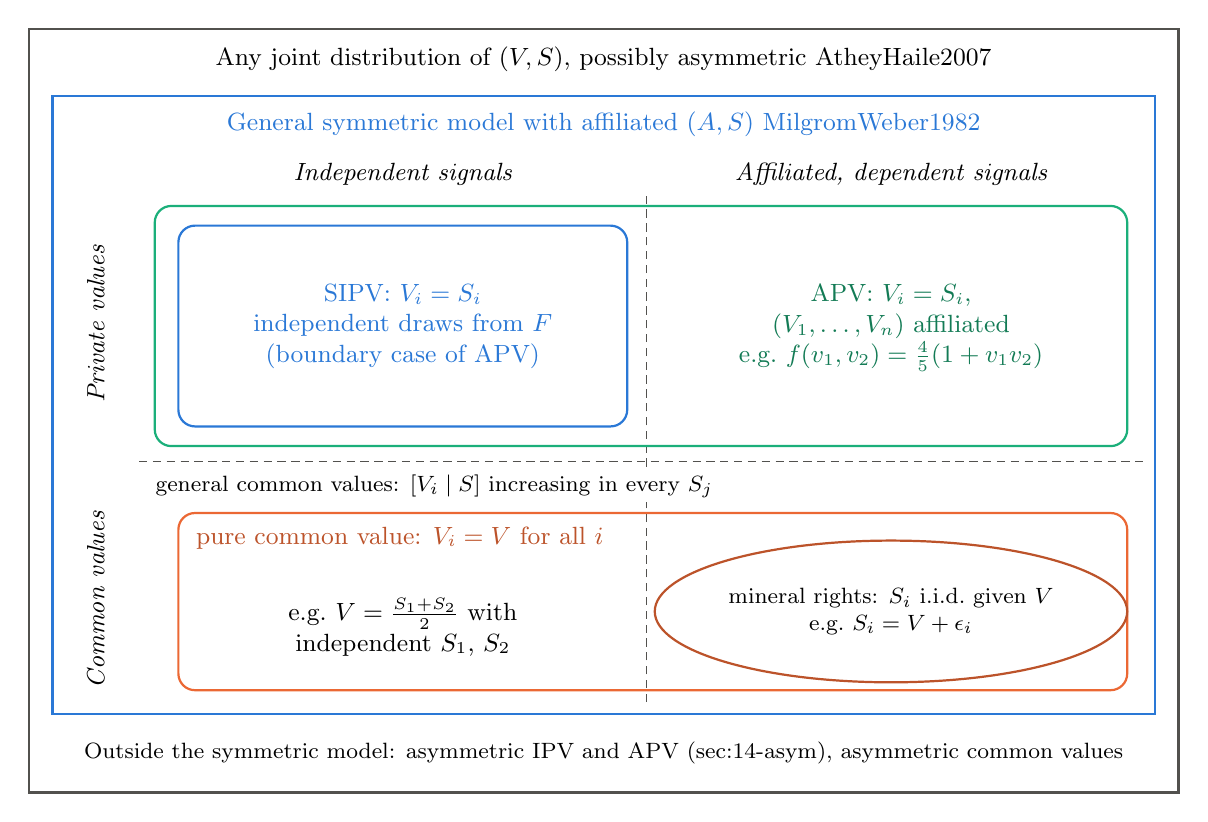
\begin{tikzpicture}[x=1cm,y=1cm,font=\small]
  \draw[thick,c14gray] (0,0) rectangle (14.6,9.7);
  \node[align=center,anchor=north] at (7.3,9.6) {Any joint distribution of $(\bm V,\bm S)$, possibly
  asymmetric \citep{AtheyHaile2007}};
  \draw[thick,c14blue] (0.3,1.0) rectangle (14.3,8.85);
  \node[align=center,anchor=north,c14blue,text width=13.4cm] at (7.3,8.77) {General symmetric model with
  affiliated $(\bm A,\bm S)$ \citep{MilgromWeber1982}};
  \node[align=center,font=\small\itshape] at (4.75,7.85) {Independent signals};
  \node[align=center,font=\small\itshape] at (10.95,7.85) {Affiliated, dependent signals};
  \node[rotate=90,font=\small\itshape] at (0.85,5.95) {Private values};
  \node[rotate=90,font=\small\itshape] at (0.85,2.45) {Common values};
  \draw[densely dashed,c14gray] (7.85,1.15) -- (7.85,7.6);
  \draw[densely dashed,c14gray] (1.4,4.2) -- (14.15,4.2);
  \draw[rounded corners=6pt,thick,c14aqua] (1.6,4.4) rectangle (13.95,7.45);
  \node[align=center,c14aqua!70!black] at (10.95,5.9) {APV: $V_i=S_i$,\\ $(V_1,\dots,V_n)$ affiliated\\
  e.g.\ $f(v_1,v_2)=\frac{4}{5}(1+v_1v_2)$};
  \draw[rounded corners=6pt,thick,c14blue] (1.9,4.65) rectangle (7.6,7.2);
  \node[align=center,c14blue] at (4.75,5.92) {SIPV: $V_i=S_i$\\ independent draws from $F$\\ (boundary case of
  APV)};
  \node[align=left,anchor=north west,font=\footnotesize,fill=white,inner sep=1.5pt] at (1.55,4.1) {general
  common values: $\E[V_i\mid\bm S]$ increasing in every $S_j$};
  \draw[rounded corners=6pt,thick,c14orange] (1.9,1.3) rectangle (13.95,3.55);
  \node[align=left,anchor=north west,c14orange!80!black] at (2.0,3.5) {pure common value: $V_i=V$ for all $i$};
  \node[align=center] at (4.75,2.1) {e.g.\ $V=\frac{S_1+S_2}{2}$ with\\ independent $S_1$, $S_2$};
  \draw[thick,c14orange!80!black] (10.95,2.3) ellipse (3.0 and 0.9);
  \node[align=center,font=\footnotesize] at (10.95,2.3) {mineral rights: $S_i$ i.i.d.\ given $V$\\ e.g.\
  $S_i=V+\epsilon_i$};
  \node[align=center,font=\footnotesize] at (7.3,0.5) {Outside the symmetric model: asymmetric IPV and APV
  (\cref{sec:14-asym}), asymmetric common values};
\end{tikzpicture}
\caption{A map of information structures. Columns separate independent from affiliated signals, and rows
separate private from common values. Independence is the boundary case of affiliation, so SIPV lies inside
APV. Pure common values can have independent or dependent signals. The mineral rights model has dependent
signals. All symmetric models with affiliated signals and values are special cases of the general model of
\citet{MilgromWeber1982}.}
\label{fig:14-taxonomy}
\end{figure}

\begin{table}[htbp]
\centering
\caption{Information structures: definitions and canonical examples}\label{tab:14-info}
\small
\begin{tabularx}{\textwidth}{@{}>{\raggedright\arraybackslash}p{2.9cm}>{\raggedright\arraybackslash}X>{\raggedright\arraybackslash}X@{}}
\toprule
Model & Definition & Example \\
\midrule
SIPV & $V_i=S_i$, values i.i.d.\ with CDF $F$ & nondurable consumer goods bought for own use
\citep[p.~1093]{MilgromWeber1982} \\
\addlinespace
IPV (asymmetric) & $V_i=S_i$, values independent with CDFs $F_i$ & timber tracts sold to mills and loggers with
different costs \citep{AtheyLevinSeira2011} \\
\addlinespace
APV & $V_i=S_i$, $(V_1,\dots,V_n)$ affiliated & a painting bought for own enjoyment by bidders with correlated
tastes \citep[p.~1099]{MilgromWeber1982} \\
\addlinespace
Common values & $\E[V_i\mid\bm S]$ strictly increasing in every $S_j$ & timber: private cost differences
plus private estimates of timber quality, volume and future market conditions
\citep[Section~II.F]{AtheyLevinSeira2011} \\
\addlinespace
Pure common value & $V_i=V$ for all $i$ & oil, gas and mineral rights \citep[Section~2.2]{MilgromWeber1982} \\
\addlinespace
Mineral rights & pure common value, $S_i$ i.i.d.\ given $V$ & offshore oil tract with independent seismic
estimates \citep[p.~1094]{MilgromWeber1982} \\
\addlinespace
General symmetric model & $V_i=u(\bm A,S_i,\bm S_{-i})$, $u$ symmetric, $(\bm A,\bm S)$ affiliated & a painting
with resale value, prestige and uncertain authenticity \citep[Section~2.3]{MilgromWeber1982} \\
\bottomrule
\end{tabularx}
\end{table}

Which structure fits a market is an empirical judgment. \citet[p.~1093]{MilgromWeber1982} argue that the
private values assumption is most nearly satisfied in auctions of nondurable consumer goods, whose
consumption is a personal matter. Mineral rights are the canonical common-value case. The value of an oil
tract depends on the unknown amount of recoverable oil, its quality, the ease of recovery and future
prices. To a first approximation these are the same for all bidders, while their estimates differ \citep[pp.~1093--1094]{MilgromWeber1982}.
\citet[Section~7]{AtheyHaile2007} add that common values arise whenever the good is not consumed
immediately and bidders have different information about future market conditions. They also arise when
bidders run their own surveys, or process the same public data with different methods. Many markets mix
both elements. In timber auctions, differences in bidders' costs and contractual arrangements create
private value differences. Bidders also form private estimates of the quality and quantity of timber and
may disagree about future market conditions. This adds a potential common value component
\citep[Section~II.F]{AtheyLevinSeira2011}. Resale opportunities can create common values even when final
consumption values are private \citep{Haile2001}. In Haile's model of timber auctions, a bidder's value
includes the option to resell the contract or to buy timber afterward in an active secondary market.
The losing bidders are potential buyers at resale, so rivals' information matters for each bidder's
value. Resale makes the prices at which bidders drop out rise with the number of bidders. Under common
values the winner's curse makes them fall \citep[Section~2.6.4, p.~100]{HortacsuPerrigne2021}.

\subsection{Affiliation}\label{sec:14-affiliation}

Most results on interdependent values require that signals and values be positively related in a strong
sense, called affiliation. For vectors $\bm z,\bm z'\in\R^k$, write $\bm z\vee\bm z'$ for their
component-wise maximum and $\bm z\wedge\bm z'$ for their component-wise minimum.

\begin{definition}[Affiliation]\label{def:14-affiliation}
Random variables $\bm Z=(Z_1,\dots,Z_k)$ with joint density $f$ are \emph{affiliated} if, for all
$\bm z,\bm z'\in\R^k$,
\begin{equation}\label{eq:14-affil-ineq}
f(\bm z\vee\bm z')\,f(\bm z\wedge\bm z')\ \ge\ f(\bm z)\,f(\bm z').
\end{equation}
\end{definition}

Inequality \eqref{eq:14-affil-ineq} is also known as the FKG inequality and as the MTP$_2$ property
(multivariate total positivity of order two). Roughly, it says that large values of some of the variables
make the other variables more likely to be large than small \citep[p.~1098]{MilgromWeber1982}. To see
this, take $k=2$, $\bm z=(x',y)$ and $\bm z'=(x,y')$ with $x'>x$ and $y'>y$. Then $\bm z\vee\bm z'=(x',y')$
and $\bm z\wedge\bm z'=(x,y)$, and \eqref{eq:14-affil-ineq} reads
\begin{equation}\label{eq:14-affil-2d}
f(x',y')\,f(x,y)\ \ge\ f(x',y)\,f(x,y').
\end{equation}
Pairs of points in which both coordinates move together are at least as likely as pairs in which they move
in opposite directions. When $\bm z$ and $\bm z'$ are ordered, say $\bm z\le\bm z'$, we have
$\bm z\vee\bm z'=\bm z'$ and $\bm z\wedge\bm z'=\bm z$, so \eqref{eq:14-affil-ineq} holds with equality.
Only unordered pairs impose restrictions. Taking logarithms shows that affiliation means that $\ln f$ is
\emph{supermodular},
\[
\ln f(\bm z\vee\bm z')+\ln f(\bm z\wedge\bm z')\ \ge\ \ln f(\bm z)+\ln f(\bm z').
\]
\Cref{sec:B-affiliation} restates the definition for reference, together with a version that does not
require densities. The next result makes the condition easy to check.

\begin{proposition}[Characterization of affiliation]\label{prop:14-affil-char}
Let $f:\R^k\to\R$ be a density.
\begin{enumerate}[label=(\roman*)]
  \item If $f$ is strictly positive and twice continuously differentiable, then $f$ is affiliated if and only
  if $\frac{\partial^2\ln f}{\partial z_i\,\partial z_j}\ge 0$ for all $i\neq j$.
  \item If $f(\bm z)=g(\bm z)h(\bm z)$, where $g$ and $h$ are nonnegative functions that satisfy
  \eqref{eq:14-affil-ineq}, then $f$ is affiliated.
\end{enumerate}
\end{proposition}

\begin{proof}
Part (ii) follows by multiplying the inequalities for $g$ and $h$, which is legitimate because both sides
are nonnegative:
\begin{align*}
f(\bm z\vee\bm z')f(\bm z\wedge\bm z')
&=\bigl[g(\bm z\vee\bm z')g(\bm z\wedge\bm z')\bigr]\bigl[h(\bm z\vee\bm z')h(\bm z\wedge\bm z')\bigr]\\
&\ge g(\bm z)g(\bm z')\,h(\bm z)h(\bm z')\\
&=f(\bm z)f(\bm z').
\end{align*}

For part (i), consider first the bivariate case $k=2$ with $\bm z=(x,y)$. Suppose that
$\frac{\partial^2\ln f}{\partial x\,\partial y}\ge 0$ everywhere. Ordered pairs satisfy
\eqref{eq:14-affil-ineq} with equality. For an unordered pair, relabel so that $\bm z=(x',y)$ and
$\bm z'=(x,y')$ with $x'>x$ and $y'>y$. Taking logarithms in \eqref{eq:14-affil-2d}, we must show that
\[
\Delta\equiv\ln f(x',y')-\ln f(x,y')-\ln f(x',y)+\ln f(x,y)\ \ge\ 0.
\]
Apply the fundamental theorem of calculus first in the first argument,
\[
\Delta=\int_x^{x'}\left[\frac{\partial\ln f(a,y')}{\partial a}-\frac{\partial\ln f(a,y)}{\partial a}\right]da,
\]
and then in the second argument,
\[
\Delta=\int_x^{x'}\!\!\int_y^{y'}\frac{\partial^2\ln f(a,c)}{\partial a\,\partial c}\,dc\,da\ \ge\ 0.
\]
Conversely, suppose $f$ is affiliated. Then $\Delta\ge 0$ for all $x'>x$ and $y'>y$. Divide $\Delta$ by
$(x'-x)(y'-y)$ and let $x'\to x$ and $y'\to y$. By the double-integral representation and the continuity of
the cross partial, the limit is $\frac{\partial^2\ln f(x,y)}{\partial x\,\partial y}$, which is therefore
nonnegative.

For $k>2$, the ``only if'' direction follows from the same argument applied to any pair of coordinates
$(z_i,z_j)$ with the other coordinates held fixed. The ``if'' direction uses a result of
\citet[p.~310]{Topkis1978}: a twice continuously differentiable function on a product of intervals is
supermodular if and only if all its cross partials are nonnegative. Applied to $\ln f$, this gives part (i)
\citep[p.~1098]{MilgromWeber1982}.
\end{proof}

For two variables, affiliation is equivalent to a familiar property of conditional densities, and it
implies a chain of stochastic orderings.

\begin{proposition}[Affiliation, likelihood ratios and stochastic dominance]\label{prop:14-affil-mlrp}
Let $(X,Z)$ have a strictly positive joint density $f(x,z)$ on $[\underline x,\bar x]\times[\underline z,\bar
z]$, with marginal density $f_Z$, conditional density $f(x\mid z)$ and conditional CDF $F(x\mid z)$.
\begin{enumerate}[label=(\roman*)]
  \item $(X,Z)$ are affiliated if and only if $f(x\mid z)$ has the \emph{monotone likelihood ratio property}
  (MLRP): for all $z'>z$, the ratio $\frac{f(x\mid z')}{f(x\mid z)}$ is nondecreasing in $x$.
  \item If $(X,Z)$ are affiliated, then the ratio $\frac{F(x\mid z)}{f(x\mid z)}$ is nonincreasing in $z$
  and the hazard rate $\frac{f(x\mid z)}{1-F(x\mid z)}$ is nonincreasing in $z$, for every $x$.
  \item If $(X,Z)$ are affiliated, then $F(x\mid z')\le F(x\mid z)$ for all $x$ and all $z'>z$. Equivalently,
  $\Pr(X\ge x\mid Z=z)$ is nondecreasing in $z$.
\end{enumerate}
\end{proposition}

\begin{proof}
(i) For two variables the only restrictions in \eqref{eq:14-affil-ineq} come from unordered pairs, so
affiliation is the inequality $f(x',z')f(x,z)\ge f(x,z')f(x',z)$ for all $x'>x$ and $z'>z$. Divide both
sides by $f_Z(z)f_Z(z')>0$:
\[
f(x'\mid z')\,f(x\mid z)\ \ge\ f(x\mid z')\,f(x'\mid z).
\]
Divide by $f(x'\mid z)f(x\mid z)>0$:
\[
\frac{f(x'\mid z')}{f(x'\mid z)}\ \ge\ \frac{f(x\mid z')}{f(x\mid z)}.
\]
This is the MLRP. Each step can be reversed, which gives the converse \citep[footnote~16]{MilgromWeber1982}.

(ii) Fix $z'>z$ and $x$. For every $t\le x$, the MLRP gives $\frac{f(t\mid z')}{f(t\mid z)}\le\frac{f(x\mid
z')}{f(x\mid z)}$, that is,
\[
f(t\mid z')\,f(x\mid z)\ \le\ f(x\mid z')\,f(t\mid z).
\]
Integrate both sides over $t\in[\underline x,x]$:
\[
F(x\mid z')\,f(x\mid z)\ \le\ f(x\mid z')\,F(x\mid z).
\]
Rearranging gives $\frac{F(x\mid z')}{f(x\mid z')}\le\frac{F(x\mid z)}{f(x\mid z)}$. For the hazard rate,
use $t\ge x$ instead. The MLRP gives $f(t\mid z')f(x\mid z)\ge f(x\mid z')f(t\mid z)$. Integrating over
$t\in[x,\bar x]$ gives $\bigl[1-F(x\mid z')\bigr]f(x\mid z)\ge f(x\mid z')\bigl[1-F(x\mid z)\bigr]$, which
rearranges to $\frac{f(x\mid z')}{1-F(x\mid z')}\le\frac{f(x\mid z)}{1-F(x\mid z)}$.

(iii) By part (ii), for every $t$,
\[
\frac{d}{dt}\ln F(t\mid z')=\frac{f(t\mid z')}{F(t\mid z')}\ \ge\ \frac{f(t\mid z)}{F(t\mid z)}=\frac{d}{dt}\ln
F(t\mid z).
\]
Integrate from $x$ to $\bar x$ and use $F(\bar x\mid z')=F(\bar x\mid z)=1$:
\[
-\ln F(x\mid z')\ \ge\ -\ln F(x\mid z).
\]
Hence $F(x\mid z')\le F(x\mid z)$, and $\Pr(X\ge x\mid Z=z)=1-F(x\mid z)$ is nondecreasing in $z$.
\end{proof}

The proposition gives the chain
\begin{align*}
\text{affiliation}&\iff\text{MLRP}\\
&\implies\text{reverse hazard rate dominance and hazard rate dominance}\\
&\implies\text{first-order stochastic dominance}.
\end{align*}
None of the converse implications holds in general. Part (iii) is the sense in which a high value of $Z$ is
good news about $X$. The step from part (ii) to part (iii) reappears in \cref{sec:14-asym}, where reverse
hazard rate dominance (\cref{def:14-rhr}) compares strong and weak bidders. A version of part (ii) for the
highest rival signal is a lemma of \citet{MilgromWeber1982} (\cref{lem:14-mw-lemma1}).

\begin{example}[Affiliated and non-affiliated densities]\label{ex:14-affil}
\leavevmode
\begin{enumerate}[label=(\alph*)]
  \item \emph{Independence.} If $f(\bm z)=\prod_{i}f_i(z_i)$, then \eqref{eq:14-affil-ineq} holds with
  equality, because the two sides contain the same factors $f_i(z_i)$ and $f_i(z_i')$. Independent
  variables are always affiliated \citep[p.~1099]{MilgromWeber1982}, and the IPV model is the boundary case
  of the APV model.
  \item \emph{Mineral rights.} Let $V$ have density $h$, and let the signals be i.i.d.\ given $V$ with
  conditional density $g(s\mid v)$. The joint density is $f(v,\bm s)=h(v)\prod_{i=1}^{n}g(s_i\mid v)$.
  Suppose $g$ has the MLRP, so that $g(s\mid v)$ satisfies the affiliation inequality in $(s,v)$. As a
  function of the whole vector $(v,\bm s)$, each factor $g(s_i\mid v)$ depends on two coordinates in which it
  satisfies \eqref{eq:14-affil-ineq}. Because $\vee$ and $\wedge$ act coordinate by coordinate, it satisfies
  \eqref{eq:14-affil-ineq} on the whole vector. The factor $h(v)$ depends on one coordinate and satisfies it
  trivially. By \cref{prop:14-affil-char}(ii), $f$ is affiliated \citep[p.~1099]{MilgromWeber1982}.
  \item \emph{Normal signals.} Let $S_i=V+\epsilon_i$ with $\epsilon_i\sim N(0,\sigma^2)$ independent of $V$.
  Then $\ln g(s\mid v)=\text{const}-\frac{(s-v)^2}{2\sigma^2}$, so $\frac{\partial^2\ln g}{\partial s\,\partial
  v}=\frac{1}{\sigma^2}>0$. The MLRP holds, and by part (b) $(V,\bm S)$ are affiliated for any prior
  density of $V$. More generally, let $\bm Z\sim N(\bm\mu,\Sigma)$. Then $\ln f(\bm
  z)=\text{const}-\frac{1}{2}(\bm z-\bm\mu)^{\T}\Sigma^{-1}(\bm z-\bm\mu)$, and
  \[
  \frac{\partial^2\ln f}{\partial z_i\,\partial z_j}=-\bigl(\Sigma^{-1}\bigr)_{ij}.
  \]
  A normal vector is affiliated if and only if every off-diagonal element of the precision matrix
  $\Sigma^{-1}$ is nonpositive. For $k=2$ with standard deviations $\sigma_x,\sigma_y$ and correlation
  $\rho$, the cross partial equals $\frac{\rho}{(1-\rho^2)\sigma_x\sigma_y}$. The pair is affiliated if and
  only if $\rho\ge 0$, so a negatively correlated normal pair is not affiliated. For $k\ge 3$, nonnegative
  correlations are not enough, because the condition concerns partial correlations.
  \item \emph{A polynomial density.} Let $(S_1,S_2)$ have density
  \begin{equation}\label{eq:14-apv-density}
  f(s_1,s_2)=\frac{4}{5}\,(1+s_1s_2)\qquad\text{on }[0,1]^2.
  \end{equation}
  It integrates to one, since $\int_0^1\!\int_0^1(1+s_1s_2)\,ds_1\,ds_2=1+\frac{1}{4}=\frac{5}{4}$. The cross
  partial of the log density is
  \[
  \frac{\partial^2}{\partial s_1\,\partial s_2}\ln(1+s_1s_2)=\frac{\partial}{\partial
  s_2}\left[\frac{s_2}{1+s_1s_2}\right]=\frac{(1+s_1s_2)-s_2s_1}{(1+s_1s_2)^2}=\frac{1}{(1+s_1s_2)^2}>0,
  \]
  so the density is affiliated. The marginal density of $S_1$ is $\frac{4}{5}\bigl(1+\frac{s_1}{2}\bigr)$,
  the conditional density is $f(s_2\mid s_1)=\frac{2(1+s_1s_2)}{2+s_1}$, and the conditional CDF is
  \[
  F(s_2\mid s_1)=\frac{s_2(2+s_1s_2)}{2+s_1},\qquad
  \frac{\partial F(s_2\mid s_1)}{\partial s_1}=\frac{2s_2(s_2-1)}{(2+s_1)^2}\le 0.
  \]
  As \cref{prop:14-affil-mlrp}(iii) requires, a higher $s_1$ shifts the distribution of $S_2$ up. For
  example, $F(\frac{1}{2}\mid s_1)$ equals $\frac{1}{2}$, $\frac{9}{20}$ and $\frac{5}{12}$ at $s_1=0$,
  $\frac{1}{2}$ and $1$. With $V_i=S_i$ this is an APV model, which \cref{sec:14-mw-eq,sec:14-mw-rank} use
  as a running example. \Cref{fig:14-affil-example} plots the density and the conditional CDFs.
\end{enumerate}
\end{example}

\begin{figure}[htbp]
\centering
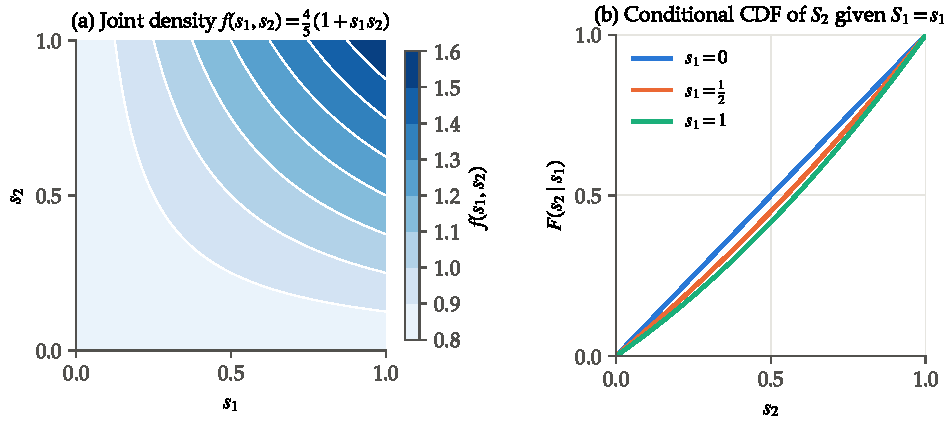
\includegraphics[width=\textwidth]{figures/ch14/affil_example.pdf}
\caption{The affiliated density $f(s_1,s_2)=\frac{4}{5}(1+s_1s_2)$ of \cref{ex:14-affil}(d). Panel (a): the
density is highest where both signals are high. Panel (b): the conditional CDF of $S_2$ shifts down as
$s_1$ rises, so a high signal for one bidder makes high signals of the other more likely.}
\label{fig:14-affil-example}
\end{figure}

Affiliation also has a probabilistic meaning that explains why it is the right condition for auction
theory. Call a set $A\subseteq\R^k$ \emph{increasing} if its indicator function is nondecreasing. Random
variables $\bm Z$ are \emph{associated} if $\Pr(\bm Z\in A\cap B)\ge\Pr(\bm Z\in A)\Pr(\bm Z\in B)$ for all
increasing sets $A$ and $B$. A set $\mathcal{S}\subseteq\R^k$ is a \emph{sublattice} if $\bm z\vee\bm z'$ and
$\bm z\wedge\bm z'$ belong to $\mathcal{S}$ whenever $\bm z$ and $\bm z'$ do. Rectangles and order intervals
$\{\bm z:\bm a\le\bm z\le\bm b\}$ are sublattices. The general definition in the appendix of
\citet{MilgromWeber1982} calls $\bm Z$ affiliated if it is associated conditional on every sublattice. For
variables with a density this coincides with \cref{def:14-affiliation} \citep[Theorem~24]{MilgromWeber1982}.

\begin{proposition}[Association and the covariance inequality]\label{prop:14-association}
\leavevmode
\begin{enumerate}[label=(\alph*)]
  \item The following statements are equivalent \citep[Theorem~22]{MilgromWeber1982}.
  \begin{enumerate}[label=(\roman*)]
    \item $\bm Z$ is associated.
    \item For every pair of nondecreasing functions $g$ and $h$, $\E[g(\bm Z)h(\bm Z)]\ge\E[g(\bm Z)]\,\E[h(\bm
    Z)]$.
    \item For every nondecreasing function $g$ and increasing set $A$, $\E[g(\bm Z)\mid A]\ge\E[g(\bm
    Z)]\ge\E[g(\bm Z)\mid \bar A]$, where $\bar A$ is the complement of $A$.
  \end{enumerate}
  \item $\bm Z$ is affiliated if and only if (ii) and (iii) hold conditional on every sublattice
  $\mathcal{S}$ \citep[Theorem~23]{MilgromWeber1982}. That is, $\E[gh\mid\mathcal{S}]\ge\E[g\mid\mathcal{S}]\,
  \E[h\mid\mathcal{S}]$ and $\E[g\mid A\cap\mathcal{S}]\ge\E[g\mid\mathcal{S}]\ge\E[g\mid\bar A\cap\mathcal{S}]$.
\end{enumerate}
\end{proposition}

\begin{proof}[Proof sketch for part (a)]
To show that (i) implies (ii), take $g$ and $h$ nonnegative and bounded. For a positive integer $K$, define
the step function
\[
g_K(\bm z)=\frac{1}{K}\sum_{l\ge 1}\indic\Bigl\{g(\bm z)>\frac{l}{K}\Bigr\},
\]
which satisfies $g(\bm z)-\frac{1}{K}\le g_K(\bm z)\le g(\bm z)$. Each set $A_l=\{\bm z:g(\bm z)>\frac{l}{K}\}$ is
increasing. Define $h_K$ and increasing sets $B_{l'}$ in the same way. Association gives
\[
\E[g_Kh_K]=\frac{1}{K^2}\sum_{l}\sum_{l'}\Pr(A_l\cap B_{l'})\ \ge\
\frac{1}{K^2}\sum_{l}\sum_{l'}\Pr(A_l)\Pr(B_{l'})=\E[g_K]\,\E[h_K].
\]
Letting $K\to\infty$ proves (ii) for nonnegative bounded functions, and the extension to general $g$ and $h$ is
routine. To show that (ii) implies (iii), take $h=\indic_A$. Then $\E[g\indic_A]\ge\E[g]\Pr(A)$, which is
$\E[g\mid A]\ge\E[g]$. The second inequality follows because $\E[g]=\Pr(A)\E[g\mid A]+\Pr(\bar A)\E[g\mid \bar
A]$ is a weighted average. To show that (iii) implies (i), take $g=\indic_B$. Then $\Pr(B\mid A)\ge\Pr(B)$,
which is association \citep[p.~1119]{MilgromWeber1982}.
\end{proof}

Part (a)(ii) says that nondecreasing functions of affiliated variables are positively correlated. Part (b)
says this remains true conditional on order-interval events, such as the event that the highest rival
signal lies below one's own. This is the form in which affiliation enters equilibrium analysis. The
properties of affiliation used most often are collected next. Write $Y_1\ge Y_2\ge\dots\ge Y_{n-1}$ for the
signals of bidder 1's rivals arranged in decreasing order, so that $Y_1=\max_{j\neq 1}S_j$.

\begin{proposition}[Properties of affiliated variables]\label{prop:14-affil-props}
Let $\bm Z=(Z_1,\dots,Z_k)$ be affiliated.
\begin{enumerate}[label=(\roman*)]
  \item If $g_1,\dots,g_k$ are all nondecreasing or all nonincreasing, then $g_1(Z_1),\dots,g_k(Z_k)$ are
  affiliated \citep[Theorem~3]{MilgromWeber1982}.
  \item Every subvector of $\bm Z$ is affiliated. In particular $Z_1,\dots,Z_{k-1}$ are affiliated
  \citep[Theorem~4]{MilgromWeber1982}.
  \item For every nondecreasing function $H$, the function
  \[
  h(a_1,b_1;\dots;a_k,b_k)=\E\bigl[H(\bm Z)\mid a_1\le Z_1\le b_1,\dots,a_k\le Z_k\le b_k\bigr]
  \]
  is nondecreasing in all its arguments. In particular, $\E[H(\bm Z)\mid Z_1=z_1,\dots,Z_l=z_l]$ is
  nondecreasing in $(z_1,\dots,z_l)$ for each $l=1,\dots,k$ \citep[Theorem~5]{MilgromWeber1982}.
  \item Under \cref{ass:14-mw}, the variables $A_1,\dots,A_m,S_1,Y_1,\dots,Y_{n-1}$ are affiliated
  \citep[Theorem~2]{MilgromWeber1982}.
\end{enumerate}
\end{proposition}

\begin{proof}
Parts (i) and (ii) follow from \cref{prop:14-association}(b)(ii), and part (iii) follows from
\cref{prop:14-association}(b)(iii) \citep[p.~1119]{MilgromWeber1982}. \Cref{sec:14-mw-affil} gives the
arguments. For part (iv), note first that the symmetry of $f$ in the signals implies that the joint density
of $(\bm A,S_1,Y_1,\dots,Y_{n-1})$ is
\begin{equation}\label{eq:14-joint-orderstat}
(n-1)!\;f(\bm a,s_1,y_1,\dots,y_{n-1})\;\indic\{y_1\ge y_2\ge\dots\ge y_{n-1}\}
\end{equation}
\citep[eq.~(4)]{MilgromWeber1982}. The factor $(n-1)!$ counts the orderings of the rivals' signals that
produce the same ordered vector, each of which has the same density by symmetry. The density $f$ is
affiliated by \cref{ass:14-mw}(v). The indicator of any sublattice satisfies \eqref{eq:14-affil-ineq}. If
both points lie in the sublattice, both sides equal one, and otherwise the right side is zero. The set
$\{y_1\ge\dots\ge y_{n-1}\}$ is a sublattice, because the component-wise maximum and minimum of two
nonincreasing sequences are nonincreasing. By \cref{prop:14-affil-char}(ii) the product
\eqref{eq:14-joint-orderstat} is affiliated.
\end{proof}

Parts (iii) and (iv) together imply that $\E[V_1\mid S_1=s,Y_1=y_1,\dots,Y_{n-1}=y_{n-1}]$ is nondecreasing in
all its arguments \citep[p.~1100]{MilgromWeber1982}. In particular, the expected value of the object to
bidder 1 conditional on its own signal and on the highest rival signal,
$v(s,y)=\E[V_1\mid S_1=s,Y_1=y]$, is nondecreasing in both arguments. \Cref{prop:14-mw-spa} shows that $v(s,s)$
is the equilibrium bid in the second-price auction with affiliated values. \Cref{app:math} collects these
results with the other mathematical tools of the book.

\subsection{The winner's curse}\label{sec:14-winners-curse}

Suppose bidders form conditionally independent estimates of a common value $V$, and each estimate is
unbiased. Other things being equal, the bidder with the largest estimate makes the highest bid. The winner
therefore tends to be the bidder who overestimated the value the most. On average, the winner finds that it
had overestimated $V$ \citep[p.~1094]{MilgromWeber1982}. This phenomenon is the \emph{winner's curse}.
Petroleum engineers \citet{CapenClappCampbell1971} claimed that it was responsible for the low profits that
oil companies earned on offshore tracts in the 1960s \citep[p.~1094]{MilgromWeber1982}.

In equilibrium the winner's curse concerns information, and rational bidders do not lose money because of
it. Winning reveals to the winner that its signal was more optimistic than its rivals' signals. This
revelation is ``bad news'' about the value of the object \citep{Milgrom1981}. Rational bidders anticipate it
and condition their bids on the event of winning. The presence of a winner's curse therefore does not imply
that winners regret winning \citep[footnote~7]{AtheyHaile2007}. Losses arise for naive bidders who ignore the
information contained in winning.

The following result makes the bad news precise in the general symmetric model. Recall that
$v(s,y)=\E[V_1\mid S_1=s,Y_1=y]$. In a symmetric equilibrium with a strictly increasing bid function, bidder 1
wins exactly when $Y_1<S_1$.

\begin{proposition}[The bad news in winning]\label{prop:14-wc}
Suppose \cref{ass:14-mw} holds. For every signal $s$ with $\Pr(Y_1<s\mid S_1=s)>0$,
\begin{equation}\label{eq:14-wc}
\E\bigl[V_1\mid S_1=s,\ Y_1<s\bigr]\ \le\ \min\Bigl\{v(s,s),\ \E\bigl[V_1\mid S_1=s\bigr]\Bigr\}.
\end{equation}
Both inequalities are strict if $v(s,y)$ is strictly increasing in $y$ and $\Pr(Y_1<s\mid S_1=s)<1$. Under
private values, $v(s,y)=s$ and both hold with equality.
\end{proposition}

\begin{proof}
By the law of iterated expectations,
\[
\E\bigl[V_1\mid S_1=s,\ Y_1<s\bigr]=\E\bigl[v(s,Y_1)\mid S_1=s,\ Y_1<s\bigr].
\]
By \cref{prop:14-affil-props}(iii) and (iv), $\varphi(y)\equiv v(s,y)$ is nondecreasing in $y$. All expectations
below are conditional on $S_1=s$. For $y<s$ we have $\varphi(y)\le\varphi(s)$, so
\[
\E[\varphi(Y_1)\mid Y_1<s]\ \le\ \varphi(s)=v(s,s),
\]
which is the first inequality. For $y\ge s$ we have $\varphi(y)\ge\varphi(s)$, so
$\E[\varphi(Y_1)\mid Y_1\ge s]\ge\varphi(s)\ge\E[\varphi(Y_1)\mid Y_1<s]$. The unconditional mean is a weighted
average of the two conditional means,
\begin{align*}
\E[V_1\mid S_1=s]=\E[\varphi(Y_1)]
&=\Pr(Y_1<s)\,\E[\varphi(Y_1)\mid Y_1<s]+\Pr(Y_1\ge s)\,\E[\varphi(Y_1)\mid Y_1\ge s]\\
&\ge\Pr(Y_1<s)\,\E[\varphi(Y_1)\mid Y_1<s]+\Pr(Y_1\ge s)\,\E[\varphi(Y_1)\mid Y_1< s]\\
&=\E[\varphi(Y_1)\mid Y_1<s],
\end{align*}
which is the second inequality. If $\varphi$ is strictly increasing, the inequalities between conditional
means are strict whenever both events have positive probability. Under private values,
$\E[V_1\mid S_1=s,Y_1=y]=s$ for all $y$.
\end{proof}

The proof uses affiliation only to guarantee that $v(s,y)$ is nondecreasing in $y$. Interdependence of
values is what creates the curse. In the example $V=\frac{S_1+S_2}{2}$ with independent signals,
$v(s,y)=\frac{s+y}{2}$ rises strictly with $y$, and the curse is present without any dependence between
signals.

The proposition explains why naive bidding fails. Suppose that in a first-price auction every bidder
naively bids its unconditional estimate $\E[V_1\mid S_1=s]$, which increases with $s$. Bidder 1 then wins
exactly when $Y_1<s$. Its expected profit conditional on winning is
\[
\E\bigl[V_1\mid S_1=s,\ Y_1<s\bigr]-\E\bigl[V_1\mid S_1=s\bigr]\ \le\ 0,
\]
which is strictly negative under common values. Naive bidders lose money on average whenever they win.
Equilibrium bids correct for the bad news, as \cref{sec:14-mw-eq} shows.

\begin{example}[The size of the curse with uniform errors]\label{ex:14-wc-uniform}
Consider a mineral rights model with $S_i=V+\epsilon_i$, where the errors $\epsilon_i$ are i.i.d.\ uniform on
$[-\omega,\omega]$ and independent of $V$, and $\omega>0$ is the half-width of the noise. Each signal is an
unbiased estimate, $\E[S_i-V]=0$. The highest signal is $S_{(n:n)}=V+\epsilon_{(n:n)}$. Write
$\epsilon_i=-\omega+2\omega U_i$ with $U_i$ i.i.d.\ uniform on $[0,1]$, so that
$\epsilon_{(n:n)}=-\omega+2\omega U_{(n:n)}$. The maximum of $n$ uniforms has CDF $x^n$ on $[0,1]$, so
\[
\E\bigl[U_{(n:n)}\bigr]=\int_0^1\bigl(1-x^n\bigr)\,dx=1-\frac{1}{n+1}=\frac{n}{n+1}.
\]
Therefore
\begin{equation}\label{eq:14-wc-bias}
\E\bigl[S_{(n:n)}-V\bigr]=-\omega+2\omega\,\frac{n}{n+1}=\omega\,\frac{2n-(n+1)}{n+1}=\omega\,\frac{n-1}{n+1}.
\end{equation}
The bias is zero for $n=1$, equals $\frac{\omega}{3}$ for $n=2$ and rises toward $\omega$ as $n$ grows. The
same steps with $\E[U_{(n-1:n)}]=\frac{n-1}{n+1}$, derived in \eqref{eq:14-uniform-means} below, give
$\E[S_{(n-1:n)}-V]=\omega\frac{n-3}{n+1}$. \Cref{fig:14-wc} plots both.
\end{example}

\begin{figure}[htbp]
\centering
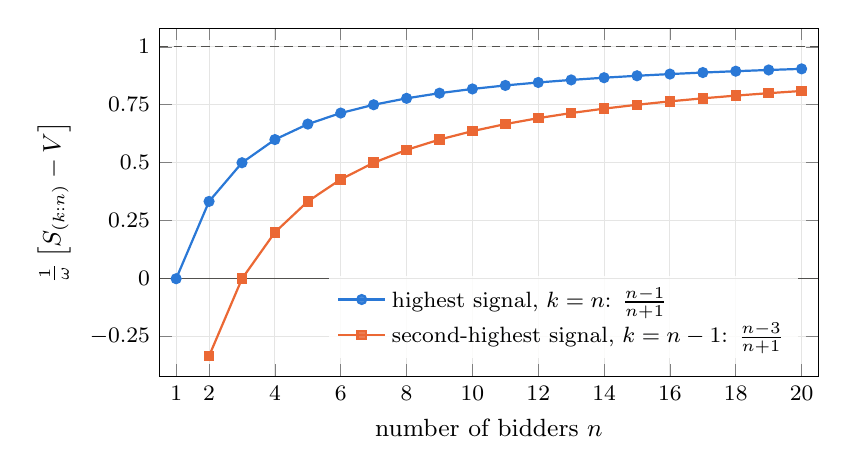
\begin{tikzpicture}
\begin{axis}[
  width=0.82\textwidth, height=6cm,
  xlabel={number of bidders $n$},
  ylabel={$\frac{1}{\omega}\,\E\bigl[S_{(k:n)}-V\bigr]$},
  xmin=0.5, xmax=20.5, ymin=-0.42, ymax=1.08,
  xtick={1,2,4,6,8,10,12,14,16,18,20},
  ytick={-0.25,0,0.25,0.5,0.75,1},
  grid=major, grid style={c14gray!15},
  legend style={at={(0.97,0.05)},anchor=south east,font=\footnotesize,draw=none,fill=white,fill opacity=0.85,text opacity=1},
  legend cell align=left,
  tick label style={font=\footnotesize}, label style={font=\small}]
\addplot[c14gray, thin, forget plot, domain=0.5:20.5] {0};
\addplot[c14gray, densely dashed, forget plot, domain=0.5:20.5] {1};
\addplot[c14blue, thick, mark=*, mark size=1.6pt, domain=1:20, samples=20] {(x-1)/(x+1)};
\addlegendentry{highest signal, $k=n$: $\frac{n-1}{n+1}$}
\addplot[c14orange, thick, mark=square*, mark size=1.5pt, domain=2:20, samples=19] {(x-3)/(x+1)};
\addlegendentry{second-highest signal, $k=n-1$: $\frac{n-3}{n+1}$}
\end{axis}
\end{tikzpicture}
\caption{The winner's curse in the mineral rights model with uniform errors on $[-\omega,\omega]$
(\cref{ex:14-wc-uniform}). Each signal is unbiased, yet the highest of $n$ signals overstates the common
value by $\omega\frac{n-1}{n+1}$ on average. The bias grows with the number of bidders and approaches
$\omega$ (dashed line).}
\label{fig:14-wc}
\end{figure}

More competition makes the bad news in winning worse. With private values, more bidders make each bidder
bid more aggressively (\cref{sec:14-fpa}). With common values, a rational bidder must also correct for a
larger bias in the event of winning. In \cref{ex:14-wc-uniform}, suppose that the prior on $V$ is
\emph{diffuse}, that is, flat over every value that the signals allow. The
second-price equilibrium bid is then $s-\omega\frac{n-2}{n}$, a correction that grows with $n$
(\cref{ex:14-mineral}). The net effect of more bidders on bids is therefore ambiguous under common values.
For the same reason, bids that fall as the number of bidders rises are a misleading test for the winner's
curse \citep{Laffont1997}. \Cref{sec:14-mw-spa} describes a sharper test based on the pivotal value.
\citet{HendricksPorter1988} test whether bidders in the drainage sales of \cref{tab:14-hp-table1} bid in a
way that accounts for the curse (\cref{ch:auction-empirics}).

\begin{remark}[Information aggregation]\label{rem:14-aggregation}
The winner's curse has a positive counterpart. It is tempting to think that the price in a mineral rights
auction conveys no more information than the winner's own estimate. This reasoning is incorrect, since the
winning estimate is the maximum of all estimates and so bounds every loser's estimate
\citep[p.~1094]{MilgromWeber1982}. Let $g(s\mid v)$ be the density of a bidder's estimate when $V=v$. Many
one-parameter families have the MLRP, so that for $v_1<v_2$ the ratio $\frac{g(s\mid v_1)}{g(s\mid v_2)}$
declines as $s$ increases. If this ratio approaches zero, the first-price price with many bidders is a
consistent estimator of $V$, even if no bidder can estimate $V$ closely on its own
\citep{Wilson1977,Milgrom1979}. Prices can thus aggregate dispersed private information.
\end{remark}

\begin{remark}[Privacy versus accuracy of information]\label{rem:14-privacy}
\citet[p.~1094]{MilgromWeber1982} stress that a bidder's expected profit in a mineral rights auction depends
more on the privacy of its information than on its accuracy. In a first-price auction, a bidder whose
information is also available to some other bidder earns zero expected profit in equilibrium
\citep{EngelbrechtWiggansMilgromWeber1983}. This logic fits the near-zero profits of the non-neighbor firms
in the drainage sales, whose information was public and therefore also known to the neighbor firms.
\Cref{prop:14-mw-garbling} proves a related result for second-price auctions.
\end{remark}

\subsection{Order statistics}\label{sec:14-orderstats}

Payments and winning probabilities in auctions are governed by order statistics of bids or values. The
winner of a second-price auction pays the second-highest bid. In a first-price auction a bidder's
probability of winning is the probability that the highest rival bid is lower than its own. This subsection
collects the facts used throughout this chapter and \cref{ch:auction-empirics}. \Cref{sec:B-orderstats}
restates them for reference and adds joint distributions and identification results.

Let $V_1,\dots,V_n$ be i.i.d.\ with continuous CDF $F$ and density $f$. Denote by $V_{(k:n)}$ the $k$-th lowest
of the $n$ draws, so that $V_{(n:n)}$ is the maximum and $V_{(n-1:n)}$ is the second highest. Denote by
$F_{(k:n)}$ its CDF. This indexing from lowest to highest follows \citet[Section~2.1]{AtheyHaile2007}.

\begin{proposition}[Distribution of an order statistic]\label{prop:14-orderstat}
For $k=1,\dots,n$,
\begin{equation}\label{eq:14-orderstat}
F_{(k:n)}(z)=\frac{n!}{(n-k)!\,(k-1)!}\int_0^{F(z)}t^{k-1}(1-t)^{n-k}\,dt,
\end{equation}
and the density of $V_{(k:n)}$ is
\begin{equation}\label{eq:14-orderstat-density}
f_{(k:n)}(z)=\frac{n!}{(n-k)!\,(k-1)!}\,F(z)^{k-1}\bigl(1-F(z)\bigr)^{n-k}f(z).
\end{equation}
\end{proposition}

\begin{proof}
The event $V_{(k:n)}\le z$ occurs if and only if at least $k$ of the $n$ draws are at most $z$. The number of
draws at most $z$ is binomial with parameters $n$ and $F(z)$. Hence
\begin{equation}\label{eq:14-orderstat-binom}
F_{(k:n)}(z)=\sum_{j=k}^{n}\binom{n}{j}F(z)^j\bigl(1-F(z)\bigr)^{n-j}.
\end{equation}
It remains to show that, for $x\in[0,1]$,
\[
\sum_{j=k}^{n}\binom{n}{j}x^j(1-x)^{n-j}=\frac{n!}{(n-k)!\,(k-1)!}\int_0^{x}t^{k-1}(1-t)^{n-k}\,dt.
\]
Both sides vanish at $x=0$, so it suffices that their derivatives agree. Using
$j\binom{n}{j}=n\binom{n-1}{j-1}$ and $(n-j)\binom{n}{j}=n\binom{n-1}{j}$, the derivative of a typical term on the
left is
\[
\frac{d}{dx}\binom{n}{j}x^j(1-x)^{n-j}=n\binom{n-1}{j-1}x^{j-1}(1-x)^{n-j}-n\binom{n-1}{j}x^{j}(1-x)^{n-j-1}.
\]
Summing over $j=k,\dots,n$, the sum telescopes. The second term for $j$ cancels the first term for $j+1$,
and the second term for $j=n$ is zero because $\binom{n-1}{n}=0$. What remains is the first term for $j=k$,
\[
n\binom{n-1}{k-1}x^{k-1}(1-x)^{n-k}=\frac{n!}{(n-k)!\,(k-1)!}\,x^{k-1}(1-x)^{n-k},
\]
which is the derivative of the right side. Formula \eqref{eq:14-orderstat-density} follows by differentiating
\eqref{eq:14-orderstat} with respect to $z$ and applying the chain rule.
\end{proof}

Formula \eqref{eq:14-orderstat} appears as equation (5) in \citet{AtheyHaile2002}. The density
\eqref{eq:14-orderstat-density} has a direct interpretation. One draw falls at $z$, $k-1$ draws fall below
and $n-k$ fall above, and the multinomial coefficient $\frac{n!}{(k-1)!\,1!\,(n-k)!}$ counts the ways of
assigning the draws to these three groups.

From bidder $i$'s point of view, the most important order statistic is the highest of its rivals' values,
$Y_1=\max_{j\neq i}V_j$. Under independence, $Y_1\le y$ if and only if every rival's value is at most $y$, so
\begin{equation}\label{eq:14-highest-rival}
F_{Y_1}(y)=F(y)^{n-1},\qquad f_{Y_1}(y)=(n-1)F(y)^{n-2}f(y).
\end{equation}
This is the case $k=n-1$ of \eqref{eq:14-orderstat} applied to the sample of $n-1$ rivals, since
$Y_1=V_{(n-1:n-1)}$ in that sample. If all bidders use the same strictly increasing bid function, a bidder
with value $v$ wins with probability $F(v)^{n-1}$.

The transaction price in second-price and ascending auctions is the second-highest value. Its CDF is
\begin{equation}\label{eq:14-second-highest}
F_{(n-1:n)}(v)=nF(v)^{n-1}\bigl(1-F(v)\bigr)+F(v)^n=\Lambda_n\bigl(F(v)\bigr),\qquad
\Lambda_n(x)\equiv nx^{n-1}(1-x)+x^n.
\end{equation}
We derive it in two ways. By counting, $V_{(n-1:n)}\le v$ if and only if at least $n-1$ of the $n$ draws are at
most $v$. Either all $n$ draws are at most $v$, with probability $F(v)^n$, or exactly $n-1$ are, with
probability $nF(v)^{n-1}(1-F(v))$. The factor $n$ counts the choices of the single draw above $v$.
Alternatively, set $k=n-1$ in \eqref{eq:14-orderstat}:
\begin{align*}
F_{(n-1:n)}(v)&=\frac{n!}{1!\,(n-2)!}\int_0^{F(v)}t^{n-2}(1-t)\,dt\\
&=n(n-1)\left[\frac{F(v)^{n-1}}{n-1}-\frac{F(v)^n}{n}\right]\\
&=nF(v)^{n-1}-(n-1)F(v)^n\\
&=nF(v)^{n-1}\bigl(1-F(v)\bigr)+F(v)^n.
\end{align*}

The map $\Lambda_n$ is a strictly increasing bijection of $[0,1]$. Indeed $\Lambda_n(0)=0$, $\Lambda_n(1)=1$,
and writing $\Lambda_n(x)=nx^{n-1}-(n-1)x^n$,
\[
\Lambda_n'(x)=n(n-1)x^{n-2}-n(n-1)x^{n-1}=n(n-1)x^{n-2}(1-x)>0\qquad\text{for }x\in(0,1).
\]
Consequently,
\begin{equation}\label{eq:14-lambda-inverse}
F(v)=\Lambda_n^{-1}\bigl(F_{(n-1:n)}(v)\bigr),
\end{equation}
so the distribution of the second-highest value determines $F$. The same argument applies to any order
statistic, because the right side of \eqref{eq:14-orderstat} is strictly increasing in $F(z)$.
\citet[Theorem~1]{AtheyHaile2002} use this fact to show that $F$ is identified from transaction prices
alone, a result developed in \cref{ch:auction-empirics}.

When $F$ is uniform on $[0,1]$, the density of $V_{(k:n)}$ is
$\frac{n!}{(n-k)!\,(k-1)!}x^{k-1}(1-x)^{n-k}$, a beta density with parameters $k$ and $n-k+1$. Using
$\int_0^1x^a(1-x)^b\,dx=\frac{a!\,b!}{(a+b+1)!}$ for nonnegative integers $a$ and $b$, its mean is
\begin{equation}\label{eq:14-uniform-means}
\E\bigl[V_{(k:n)}\bigr]=\frac{n!}{(n-k)!\,(k-1)!}\int_0^1x^{k}(1-x)^{n-k}\,dx
=\frac{n!}{(n-k)!\,(k-1)!}\cdot\frac{k!\,(n-k)!}{(n+1)!}=\frac{k}{n+1}.
\end{equation}
The $n$ draws split $[0,1]$ into $n+1$ segments of equal expected length. In particular
$\E[V_{(n:n)}]=\frac{n}{n+1}$ and $\E[V_{(n-1:n)}]=\frac{n-1}{n+1}$. \Cref{fig:14-orderstat} plots the
densities of the two highest of four uniform values, together with the density of the highest of three
rival values.

\begin{figure}[htbp]
\centering
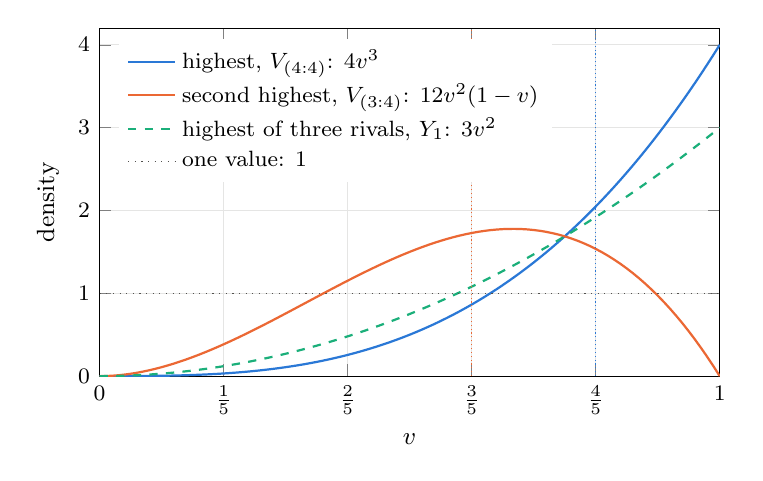
\begin{tikzpicture}
\begin{axis}[
  width=0.78\textwidth, height=6cm,
  xlabel={$v$}, ylabel={density},
  xmin=0, xmax=1, ymin=0, ymax=4.2,
  xtick={0,0.2,0.4,0.6,0.8,1},
  xticklabels={$0$,$\frac{1}{5}$,$\frac{2}{5}$,$\frac{3}{5}$,$\frac{4}{5}$,$1$},
  grid=major, grid style={c14gray!15},
  legend style={at={(0.03,0.97)},anchor=north west,font=\footnotesize,draw=none},
  legend cell align=left,
  tick label style={font=\footnotesize}, label style={font=\small}]
\addplot[c14blue, thick, domain=0:1, samples=101] {4*x^3};
\addlegendentry{highest, $V_{(4:4)}$: $4v^3$}
\addplot[c14orange, thick, domain=0:1, samples=101] {12*x^2*(1-x)};
\addlegendentry{second highest, $V_{(3:4)}$: $12v^2(1-v)$}
\addplot[c14aqua, thick, dashed, domain=0:1, samples=101] {3*x^2};
\addlegendentry{highest of three rivals, $Y_1$: $3v^2$}
\addplot[c14gray, thin, dotted, domain=0:1] {1};
\addlegendentry{one value: $1$}
\draw[c14blue, densely dotted] (axis cs:0.8,0) -- (axis cs:0.8,4.2);
\draw[c14orange, densely dotted] (axis cs:0.6,0) -- (axis cs:0.6,4.2);
\end{axis}
\end{tikzpicture}
\caption{Densities of order statistics of $n=4$ values drawn from the uniform distribution on $[0,1]$. The
vertical lines mark the means $\E[V_{(4:4)}]=\frac{4}{5}$ and $\E[V_{(3:4)}]=\frac{3}{5}$ from
\eqref{eq:14-uniform-means}. The dashed curve is the density of the highest of a bidder's three rivals,
$f_{Y_1}(v)=3v^2$, from \eqref{eq:14-highest-rival}.}
\label{fig:14-orderstat}
\end{figure}

Finally, two facts about expectations are used repeatedly. For a nonnegative random variable $X$,
$\E[X]=\int_0^\infty\Pr(X>x)\,dx$. For values supported on $[0,\bar v]$, this gives
\begin{equation}\label{eq:14-mean-second}
\E\bigl[V_{(n-1:n)}\bigr]=\int_0^{\bar v}\Bigl[1-\Lambda_n\bigl(F(v)\bigr)\Bigr]dv.
\end{equation}
When signals are dependent, the order statistics of the rivals' signals have the joint density
\eqref{eq:14-joint-orderstat}. In the descending notation of \citet{MilgromWeber1982}, $Y_k$ is the $k$-th
highest of the $n-1$ rivals' signals, which is $S_{(n-k:n-1)}$ in the ascending notation applied to the
rivals' sample.

\section{Second-Price and Ascending Auctions with Private Values}\label{sec:14-spa}

We now solve the simplest auctions in the simplest information structure. Throughout this section values
are private, so each bidder knows its own value $v_i$. The first two results allow any joint distribution
of values. The third specializes to the SIPV model to compute revenue and surplus.

\subsection{Truthful bidding in the second-price auction}\label{sec:14-spa-dominance}

Consider a second-price sealed-bid auction with reserve price $r\ge 0$. Fix bidder $i$ with value $v_i$ and
any bids of its rivals. Let
\[
\tilde m=\max\Bigl\{r,\ \max_{j\neq i}b_j\Bigr\}
\]
be the \emph{price to beat}, the lowest price at which bidder $i$ can win. By \eqref{eq:14-payoff-spa}, a
bid $b\ge r$ wins when it exceeds every rival bid, and the winner pays $\tilde m$. Bidder $i$'s payoff from
such a bid is
\begin{equation}\label{eq:14-spa-payoff}
u_i(b;\bm b_{-i})=(v_i-\tilde m)\,\indic\Bigl\{b>\max_{j\neq i}b_j\Bigr\},
\end{equation}
and its payoff from a bid below $r$ is zero. A bid above $\tilde m$ therefore wins, and a bid below
$\tilde m$ loses. A bid $b=\tilde m$ wins at price $r$ when every rival bid is below $r$. Otherwise it ties
with the highest rival bid, and \eqref{eq:14-payoff-spa} counts the tie as a loss. Any other tie-breaking
rule leaves the argument below unchanged, because a tied bid still earns either $v_i-\tilde m$ or zero.
The payment does not depend on bidder $i$'s own bid, which
only determines whether $i$ wins. A strategy is \emph{weakly dominant} if it does at least as well as any other
strategy against every profile of rivals' bids. It must also do strictly better than each alternative
against some profile. Bids below $r$ are all rejected, so we treat them as one action, not bidding.

\begin{proposition}[Vickrey 1961]\label{prop:14-spa-dominant}
With private values, bidding one's value, $b_i=v_i$, is a weakly dominant strategy in the second-price
sealed-bid auction with any reserve price. The result requires no assumption on the number of bidders, on
the joint distribution of values or on the bidder's knowledge of that distribution.
\end{proposition}

\begin{proof}
Fix the rivals' bids, and hence $\tilde m$. Every bid leads to one of two outcomes. Bidder $i$ either wins
and receives $v_i-\tilde m$, or loses and receives zero. The bid $b=v_i$ wins when $v_i>\tilde m$ and loses
when $v_i<\tilde m$. When $v_i=\tilde m$, both outcomes give zero. Hence the bid $v_i$ yields
\[
u_i(v_i;\bm b_{-i})=\max\{v_i-\tilde m,\ 0\},
\]
the larger of the two possible payoffs. No bid does better against any $\tilde m$. If $v_i<r$, the bid
$v_i$ is rejected and earns zero, which is optimal because any winning bid pays at least $r>v_i$.

Every other bid does strictly worse against some $\tilde m$, with two exceptions. For $v_i<r$, every bid
below $r$ is the same action as bidding $v_i$. For $v_i=r$, not bidding earns the same as bidding $v_i$
against every profile, so we treat the two as one action. A bid $b>v_i$ wins when
$v_i<\tilde m<b$ and then earns $v_i-\tilde m<0$, where bidding $v_i$ would have earned zero. A bid $b<v_i$
loses when $b<\tilde m<v_i$ and earns zero, where bidding $v_i$ would have earned $v_i-\tilde m>0$. Hence
$b_i=v_i$ is weakly dominant \citep{Vickrey1961}.
\end{proof}

\Cref{fig:14-spa-payoff} draws the three cases. Bidding one's value is optimal against every possible price
to beat, so a bidder needs no forecast of rivals' behavior. This is why the result needs neither symmetry,
nor independence, nor common knowledge of the distribution of values.

\begin{figure}[htbp]
\centering
\begin{tikzpicture}
\pgfplotsset{spapanel/.style={
  scale only axis, width=3.75cm, height=3.0cm, axis lines=middle, xmin=0, xmax=1.08, ymin=-0.38, ymax=0.72,
  xtick=\empty, ytick=\empty, xlabel={$\tilde m$}, xlabel style={anchor=west,font=\small},
  title style={font=\small,yshift=4pt}, clip=false}}
\begin{axis}[spapanel, name=pA, title={(a) underbidding, $b<v$}]
  \fill[c14orange!35] (axis cs:0.35,0) -- (axis cs:0.6,0) -- (axis cs:0.35,0.25) -- cycle;
  \addplot[c14gray, densely dashed, domain=0.35:0.6] {0.6-x};
  \addplot[c14blue, very thick, domain=0:0.35] {0.6-x};
  \addplot[c14blue, very thick, domain=0.35:1.0] {0};
  \node[font=\footnotesize,anchor=south west] at (axis cs:0.42,0.18) {forgone gain};
  \node[font=\footnotesize,anchor=north] at (axis cs:0.35,0) {$b$};
  \node[font=\footnotesize,anchor=north] at (axis cs:0.6,0) {$v$};
  \node[font=\small,anchor=east] at (axis cs:0,0.62) {payoff};
\end{axis}
\begin{axis}[spapanel, name=pB, at={($(pA.east)+(0.75cm,0)$)}, anchor=west, title={(b) truthful, $b=v$}]
  \addplot[c14blue, very thick, domain=0:0.6] {0.6-x};
  \addplot[c14blue, very thick, domain=0.6:1.0] {0};
  \node[font=\footnotesize,anchor=south west] at (axis cs:0.30,0.36) {$\max\{v-\tilde m,0\}$};
  \node[font=\footnotesize,anchor=north] at (axis cs:0.6,0) {$v=b$};
\end{axis}
\begin{axis}[spapanel, name=pC, at={($(pB.east)+(0.75cm,0)$)}, anchor=west, title={(c) overbidding, $b>v$}]
  \fill[c14orange!35] (axis cs:0.6,0) -- (axis cs:0.85,0) -- (axis cs:0.85,-0.25) -- cycle;
  \addplot[c14blue, very thick, domain=0:0.85] {0.6-x};
  \addplot[c14blue, very thick, domain=0.85:1.0] {0};
  \node[font=\footnotesize,anchor=north east] at (axis cs:0.6,0) {$v$};
  \node[font=\footnotesize,anchor=north] at (axis cs:0.85,-0.25) {$b$};
  \node[font=\footnotesize,anchor=west] at (axis cs:0.88,-0.14) {added loss};
\end{axis}
\end{tikzpicture}
\caption{Payoff in a second-price auction as a function of the price to beat $\tilde m$, for a bidder with
value $v$. Truthful bidding (b) attains $\max\{v-\tilde m,0\}$ for every $\tilde m$. Underbidding (a) loses
the auction when $b<\tilde m<v$ and forgoes the shaded gains. Overbidding (c) wins when $v<\tilde m<b$ and
adds the shaded losses.}
\label{fig:14-spa-payoff}
\end{figure}

\begin{remark}[What the result does and does not need]\label{rem:14-spa-needs}
The proof compares only the sign of $v_i-\tilde m$. It therefore holds for any increasing utility of money
$\mathcal{U}$ with $\mathcal{U}(0)=0$, so a risk-averse bidder also bids its value (\cref{sec:14-fpa} uses
this). The proof does require private values. With interdependent values a bidder does not know its value
when it bids, and the payoff $v_i-\tilde m$ is replaced by an expectation that depends on what winning at
price $\tilde m$ reveals. \Cref{prop:14-mw-spa} shows that the equilibrium bid then becomes $v(s,s)$.
\end{remark}

\begin{remark}[Other equilibria]\label{rem:14-spa-other}
Truthful bidding is the only weakly undominated strategy, up to the equivalence of all bids below $r$.
The second-price auction has other Bayesian Nash equilibria in weakly dominated strategies. Let values lie in $[\underline v,\bar v]$ and set
$r=\underline v$. Suppose bidder 1 bids $\bar v$ whatever its value and every other bidder bids
$\underline v$. Bidder 1 always wins and pays $\underline v\le v_1$, and no other bid gives it more. Any other
bidder could win only by bidding above $\bar v$, and would then pay $\bar v\ge v_j$. Hence no bidder gains by
deviating. This equilibrium misallocates the object whenever a rival values it more than bidder 1, and it
yields revenue $\underline v$. Following \citet[Section~2.2]{AtheyHaile2007}, we restrict attention to
equilibria in weakly undominated strategies.
\end{remark}

\begin{remark}[Second-price auctions in practice]
Pure second-price sealed-bid auctions are uncommon in practice \citep[footnote~2]{AtheyHaile2007}. The
proxy bidding system of eBay has the flavor of a second-price auction. A bidder submits a maximum, and the
system bids on its behalf up to that maximum, so the winner pays roughly the second-highest maximum. Bidders
can usually observe and respond to the bids of at least some rivals, however, as in an ascending auction.
\end{remark}

\subsection{The English auction with private values}\label{sec:14-english-pv}

The same logic solves the button auction of \cref{def:14-button}. The dynamic structure adds nothing under
private values, because a bidder has nothing to learn from rivals' exits about its own value.

\begin{proposition}[English auction with private values]\label{prop:14-english-dominant}
With private values, consider the English (button) auction with any reserve price. For each bidder, the
strategy of remaining active until the price reaches $v_i$, whatever the history of exits, is weakly
dominant. When all bidders follow it, the bidder with the highest value wins whenever that value is at
least $r$. The winner pays
\begin{equation}\label{eq:14-english-price}
P=\max\bigl\{V_{(n-1:n)},\ r\bigr\}\qquad\text{if }V_{(n:n)}\ge r,
\end{equation}
where $V_{(n:n)}$ and $V_{(n-1:n)}$ are the highest and second-highest values. If $V_{(n:n)}<r$, the object
is not sold. The second-price sealed-bid auction with truthful bids produces the same allocation and price.
\end{proposition}

\begin{proof}
Fix bidder $i$, the strategies of its rivals and the realization of the rivals' values. Rivals observe the
price and the set of active bidders. As long as bidder $i$ is active, its plans for the future do not affect
what the rivals observe. Hence the path of rival exits up to the moment bidder $i$ quits is the same for
every strategy of bidder $i$. Let $\tilde m$ be the price at which the last rival would quit along this
path. Set $\tilde m=r$ if no rival is active at the reserve price, and $\tilde m=+\infty$ if some rival never
quits. Any strategy of bidder $i$ results in some quitting price $d$ along this path, which may depend on the
rival exits it observes. Bidder $i$ wins if $d>\tilde m$ and then pays $\tilde m$, so its payoff is
\[
(v_i-\tilde m)\,\indic\{d>\tilde m\}.
\]
As in \eqref{eq:14-spa-payoff}, bidder $i$ either wins and receives $v_i-\tilde m$ or loses and receives
zero. By the argument in the proof of \cref{prop:14-spa-dominant},
quitting at $d=v_i$ yields $\max\{v_i-\tilde m,0\}$, the largest payoff available against any $\tilde m$.
This holds for every profile of rival strategies and every realization of rival values, so the strategy is
weakly dominant.

When every bidder follows this strategy, bidders quit in increasing order of their values. The auction
ends when the bidder with the second-highest value quits at price $V_{(n-1:n)}$, or at $r$ if that value is
below $r$. The bidder with the highest value wins, provided its value is at least $r$. The second-price
auction with truthful bids gives the same winner and the same price.
\end{proof}

Under private values the English and second-price auctions are therefore equivalent in a weaker sense than
strategic equivalence \citep[p.~1091]{MilgromWeber1982}. Each has a unique dominant strategy equilibrium,
and the two equilibria produce the same outcome. The equilibrium strategy is the one recorded in equation
(2.6) of \citet{AtheyHaile2007}, under which each bidder bids up to its value. The argument requires that
each bidder know its value. It fails when the value depends on what others know, as with minerals of
unknown quantity or a painting to be resold at an unknown price.

An allocation is \emph{efficient} if the object goes to the bidder who values it most. Both auctions
allocate efficiently whenever some bidder values the object above $r$. Without a reserve price the
outcome is always efficient, or Pareto optimal in the terms of \citet[p.~1091]{MilgromWeber1982}. This conclusion does not
depend on symmetry or independence. In symmetric models the Dutch and
first-price auctions also allocate efficiently. With asymmetric bidders they need not
(\cref{sec:14-asym}). Bidders also need no knowledge of rivals' value distributions or of the number of
rivals. \citet[Section~2.1]{AtheyHaile2007} note that the common knowledge assumptions are inconsequential
for ascending auctions with private values.

\subsection{Revenue and surplus with symmetric independent private values}\label{sec:14-spa-revenue}

We now compute expected revenue and bidders' expected surplus in the SIPV model. Values are i.i.d.\ with CDF
$F$ and density $f$ on $[\underline v,\bar v]$, with $\underline v\ge 0$, and the reserve price satisfies
$r\in[\underline v,\bar v]$. By \cref{prop:14-english-dominant} the formulas apply to both the second-price
and the English auction.

\begin{proposition}[Revenue and surplus in the second-price and English auctions]\label{prop:14-spa-revenue}
Consider the SIPV model with reserve price $r$.
\begin{enumerate}[label=(\roman*)]
  \item Expected revenue is
  \begin{equation}\label{eq:14-spa-revenue}
  R(r)=r\bigl[1-F(r)^n\bigr]+\int_r^{\bar v}\Bigl[1-\Lambda_n\bigl(F(v)\bigr)\Bigr]dv.
  \end{equation}
  Without a binding reserve price, $r=\underline v$, this equals
  $\E[V_{(n-1:n)}]=\underline v+\int_{\underline v}^{\bar v}\bigl[1-\Lambda_n(F(v))\bigr]dv$.
  \item A bidder with value $v\ge r$ wins with probability $Q(v)=F(v)^{n-1}$, makes the expected payment
  \begin{equation}\label{eq:14-spa-payment}
  m(v)=rF(r)^{n-1}+\int_r^{v}y\,dF(y)^{n-1}=vF(v)^{n-1}-\int_r^{v}F(y)^{n-1}\,dy,
  \end{equation}
  and earns the expected surplus
  \begin{equation}\label{eq:14-spa-surplus}
  \pi(v)=vQ(v)-m(v)=\int_r^{v}F(y)^{n-1}\,dy.
  \end{equation}
  Bidders with values below $r$ earn zero.
  \item If values are uniform on $[0,1]$, then
  \begin{equation}\label{eq:14-spa-uniform}
  R(r)=\frac{n-1}{n+1}+r^n-\frac{2n}{n+1}\,r^{n+1},\qquad \pi(v)=\frac{v^n-r^n}{n}.
  \end{equation}
  Without a reserve price, revenue is $\frac{n-1}{n+1}$, each bidder's ex ante expected surplus is
  $\frac{1}{n(n+1)}$, and total surplus is $\frac{n}{n+1}$.
\end{enumerate}
\end{proposition}

\begin{proof}
(i) The price is $P=\max\{V_{(n-1:n)},r\}$ if $V_{(n:n)}\ge r$ and zero otherwise. Since $P\ge 0$,
$\E[P]=\int_0^\infty\Pr(P>p)\,dp$. For $p<r$, $P>p$ if and only if the object is sold, that is,
$V_{(n:n)}\ge r$. This has probability $1-F(r)^n$. For $p\ge r$, $P>p$ if and only if $V_{(n-1:n)}>p$, since
$V_{(n-1:n)}>p\ge r$ already implies $V_{(n:n)}>r$. By \eqref{eq:14-second-highest} this has probability
$1-\Lambda_n(F(p))$, which is zero for $p\ge\bar v$. Hence
\[
R(r)=\int_0^{r}\bigl[1-F(r)^n\bigr]dp+\int_r^{\bar v}\Bigl[1-\Lambda_n\bigl(F(p)\bigr)\Bigr]dp,
\]
which is \eqref{eq:14-spa-revenue}. With $r=\underline v$ we have $F(r)=0$, and the first term equals
$\underline v$.

(ii) A bidder with value $v\ge r$ wins if and only if $Y_1<v$. By \eqref{eq:14-highest-rival},
$Q(v)=F(v)^{n-1}$. When it wins, it pays $\max\{Y_1,r\}$. Hence
\[
m(v)=\E\bigl[\max\{Y_1,r\}\,\indic\{Y_1<v\}\bigr]=rF(r)^{n-1}+\int_r^{v}y\,dF(y)^{n-1}.
\]
Integration by parts gives
\[
\int_r^{v}y\,dF(y)^{n-1}=vF(v)^{n-1}-rF(r)^{n-1}-\int_r^{v}F(y)^{n-1}\,dy.
\]
Substituting, $m(v)=vF(v)^{n-1}-\int_r^vF(y)^{n-1}dy$, and therefore
$\pi(v)=vF(v)^{n-1}-m(v)=\int_r^vF(y)^{n-1}dy$.

(iii) With $F(v)=v$ on $[0,1]$ we have $\Lambda_n(v)=nv^{n-1}-(n-1)v^n$. Then
\[
\int_r^1\bigl[1-\Lambda_n(v)\bigr]dv=(1-r)-(1-r^n)+\frac{n-1}{n+1}\bigl(1-r^{n+1}\bigr).
\]
Adding $r(1-r^n)$ gives
\begin{align*}
R(r)&=r-r^{n+1}+r^n-r+\frac{n-1}{n+1}-\frac{n-1}{n+1}\,r^{n+1}\\
&=\frac{n-1}{n+1}+r^n-\frac{2n}{n+1}\,r^{n+1}.
\end{align*}
With $r=0$, revenue is $\frac{n-1}{n+1}$, which matches $\E[V_{(n-1:n)}]$ in \eqref{eq:14-uniform-means}. The
surplus is $\pi(v)=\int_r^vy^{n-1}dy=\frac{v^n-r^n}{n}$. With $r=0$, the ex ante surplus is
$\E[\pi(V)]=\frac{1}{n}\int_0^1v^n\,dv=\frac{1}{n(n+1)}$. Total surplus is $\E[V_{(n:n)}]=\frac{n}{n+1}$,
because the allocation is efficient. As a check, revenue plus the surplus of all $n$ bidders is
$\frac{n-1}{n+1}+\frac{n}{n(n+1)}=\frac{n}{n+1}$.
\end{proof}

Formula \eqref{eq:14-spa-surplus} is the first appearance of a general principle. The interim surplus of a
bidder depends only on the probabilities of winning of lower types,
\[
\pi(v)=\pi(r)+\int_r^{v}Q(y)\,dy.
\]
\Cref{sec:14-ret} shows that this relation holds in every auction and is the source of revenue
equivalence.

The reserve price trades off two effects. Differentiating \eqref{eq:14-spa-uniform},
\[
R'(r)=nr^{n-1}-2nr^n=nr^{n-1}(1-2r).
\]
Revenue rises with $r$ up to $r=\frac{1}{2}$ and falls afterward, for every $n$. A higher reserve raises the
price when exactly one bidder values the object above $r$. It loses the sale when nobody does. For uniform
values, \cref{sec:14-optimal} shows that $r=\frac{1}{2}$ maximizes expected revenue among all selling
mechanisms, a result due to \citet{Myerson1981} and \citet{RileySamuelson1981}. \Cref{tab:14-spa-uniform}
evaluates the formulas of \cref{prop:14-spa-revenue} for several numbers of bidders.

\begin{table}[htbp]
\centering
\caption{Second-price and English auctions with uniform values on $[0,1]$}\label{tab:14-spa-uniform}
\small
\begin{tabular}{@{}ccccccccc@{}}
\toprule
 & \multicolumn{2}{c}{Expected revenue} & \multicolumn{2}{c}{Total surplus} &
 \multicolumn{2}{c}{Surplus per bidder} & Probability \\
\cmidrule(lr){2-3}\cmidrule(lr){4-5}\cmidrule(lr){6-7}
$n$ & $r=0$ & $r=\frac{1}{2}$ & $r=0$ & $r=\frac{1}{2}$ & $r=0$ & $r=\frac{1}{2}$ & of no sale, $r=\frac{1}{2}$ \\
\midrule
2  & 0.3333 & 0.4167 & 0.6667 & 0.5833 & 0.1667 & 0.0833 & 0.2500 \\
3  & 0.5000 & 0.5313 & 0.7500 & 0.7031 & 0.0833 & 0.0573 & 0.1250 \\
5  & 0.6667 & 0.6719 & 0.8333 & 0.8203 & 0.0333 & 0.0297 & 0.0313 \\
10 & 0.8182 & 0.8183 & 0.9091 & 0.9086 & 0.0091 & 0.0090 & 0.0010 \\
\bottomrule
\end{tabular}

\smallskip
\begin{minipage}{0.92\textwidth}
\footnotesize Notes: Computed from \cref{prop:14-spa-revenue}. Revenue is
$\frac{n-1}{n+1}+r^n-\frac{2n}{n+1}r^{n+1}$, total surplus is $\frac{n}{n+1}(1-r^{n+1})$, surplus per bidder is
$\frac{1}{n}\bigl[\frac{1-r^{n+1}}{n+1}-r^n(1-r)\bigr]$ and the probability of no sale is $r^n$. With $n=2$
the exact values are $\frac{1}{3}$ and $\frac{5}{12}$ for revenue, $\frac{2}{3}$ and $\frac{7}{12}$ for
total surplus and $\frac{1}{6}$ and $\frac{1}{12}$ for surplus per bidder.
\end{minipage}
\end{table}

Three patterns stand out in \cref{tab:14-spa-uniform}. Revenue rises and bidder surplus falls as the number
of bidders grows, because the second-highest value moves toward the highest. With two bidders, the reserve
price raises revenue from $\frac{1}{3}$ to $\frac{5}{12}$, a gain of 25 percent. Total surplus falls from
$\frac{2}{3}$ to $\frac{7}{12}$, because the object goes unsold with probability $\frac{1}{4}$. As $n$ grows,
the gain from the reserve price vanishes, since it becomes unlikely that fewer than two bidders value the
object above $r$.

\subsection{What second-price and English auctions reveal}\label{sec:14-spa-data}

The dominant strategy results have strong empirical implications, which \cref{ch:auction-empirics}
develops. In a second-price auction with private values, bids equal values. If all bids from SIPV auctions
are observed, they are i.i.d.\ draws from $F$, and their empirical distribution estimates $F$ directly. In
an English auction the winner's value is never revealed, because the auction stops when the bidder with the
second-highest value quits. The transaction price is the most reliably observed outcome. By
\eqref{eq:14-english-price} it equals $V_{(n-1:n)}$ when the reserve price does not bind. Because $\Lambda_n$ is
strictly increasing, the distribution of transaction prices in auctions with $n$ bidders determines $F$
through \eqref{eq:14-lambda-inverse} \citep[Theorem~1]{AtheyHaile2002}.

Both arguments rest on private values and on the button model. With interdependent values, bids no longer
equal values (\cref{sec:14-mw-eq}). In real open-outcry auctions, recorded bids need not equal the prices at
which bidders would quit (\cref{sec:14-formats-english}). With asymmetric independent private values,
truthful bidding remains dominant and the allocation remains efficient. Revenue is then the expected
second-highest of values drawn from different distributions (\cref{sec:14-asym}).
